\documentclass{sig-alternate}

\usepackage{graphicx}
\usepackage{balance}  % for  \balance command ON LAST PAGE  (only there!)
\usepackage[T1]{fontenc}
\usepackage{subfig,float}
%\usepackage{subfloat}
\usepackage{cite}
\graphicspath{{./figures/}{./vlfigures/}}
%graphicspath{{./vlfigures/}}
\let\proof\relax 
\let\endproof\relax
\usepackage{amsmath}
\usepackage{amsthm,amsfonts}
\usepackage{amssymb}
%\interdisplaylinepenalty=2500
\usepackage{verbatim}
\usepackage{url}
\usepackage{pbox}
\usepackage{xspace}
\usepackage{setspace}
\usepackage{tikz}
\usetikzlibrary{snakes,arrows,shapes}
\usetikzlibrary{positioning}
\usepackage{multirow}
\usepackage{caption}
\DeclareCaptionType{copyrightbox}
\usepackage{pstricks,pst-plot,pst-node,pst-grad,pstricks-add,pst-tree,pst-slpe}
\makeatletter
\newif\if@restonecol
\makeatother
\let\algorithm\relax
\let\endalgorithm\relax
\usepackage[linesnumbered,boxed,commentsnumbered]{algorithm2e}
\gdef\balancecolumns
{\vfill\eject
\global\@colht=\textheight
\global\ht\@cclv=\textheight
}

\newcommand*\Let[2]{\State #1 $\gets$ #2}
%\algrenewcommand\alglinenumber[1]{
    %{\sf\footnotesize\addfontfeatures{Colour=888888,Numbers=Monospaced}#1}}
    %\algrenewcommand\algorithmicrequire{\textbf{Precondition:}}
    %\algrenewcommand\algorithmicensure{\textbf{Postcondition:}}
%%%%%%%%%%% new for algorithm
%\floatname{algorithm}{Procedure}
%\renewcommand{\algorithmicrequire}{\textbf{Input:}}
%\renewcommand{\algorithmicensure}{\textbf{Output:}}

\newtheorem*{mydef}{Definition}
\newtheorem{thm}{Theorem}
\newtheorem{lemma}{Lemma}
\newtheorem*{myclaim}{Claim}
\newtheorem*{myproof}{Proof}

% Commands
\newcommand{\pat}{P\xspace}
\newcommand{\db}{G\xspace}
\newcommand{\vg}{V_G\xspace}
\newcommand{\eg}{E_G\xspace}
\newcommand{\vp}{V_P\xspace}
\newcommand{\ep}{E_P\xspace}
\newcommand{\Approx}{\approx}
\newcommand{\Sub}{\simeq}
\newcommand{\Iso}{\cong}
\newcommand{\khop}{k-hop\xspace}
\newcommand{\khopl}[2]{\ensuremath{h_{#1}(#2)}}
\newcommand{\nclab}[2]{\ensuremath{\eta_{#1}(#2)}}
\newcommand{\khops}{k-hops\xspace}
\newcommand{\ncl}{NL\xspace}
\newcommand{\combined}{CL\xspace}
\newcommand{\CR}{\ensuremath{R'(u)}\xspace}
\newcommand{\RS}{\ensuremath{R(u)}\xspace}
\newcommand{\cl}[2]{\ensuremath{C_{#2}(#1)}}
\newcommand{\kpath}[3]{#1\stackrel{#3}{\longrightarrow}#2}
%\newcommand{\khopcost}[3]{C_{#1}[\khopl{#1}{#2}][\khopl{#1}{#3}]}
\newcommand{\khopcost}[3]{\mathcal{C}[\khopl{#1}{#2}][\khopl{#1}{#3}]}
% equivalence between the sets
\newcommand{\Meq}{\equiv}
\newcommand{\lab}[2]{\ensuremath{L_{#2}(#1)}}
\newcommand{\Cs}{$\mathbf{M}$\xspace}
\newcommand{\M}[1]{$\mathcal{#1}$\xspace}
\newcommand{\matij}[3]{\mathcal{#1}[#2][#3]}
\newcommand{\setR}{{\mathord{\mathbb R}}}
\newcommand{\ldist}{0.3cm}
\newcommand{\putNode}[6]{\cnodeput[linecolor=black](#1,#2) {#3} {#4} \uput{\ldist}[#5](#3){ {#6} } }
\makeatother

\begin{document}

\title{\Large Approximate Graph Mining with Label
Costs~\titlenote{This work was supported in part by an HP
Innovation Award and NSF Award CCF-1240646.}}

\numberofauthors{2} 
\author{
\alignauthor
Pranay Anchuri, Mohammed J. Zaki\\
\affaddr{CS Department, RPI, Troy NY, USA}\\
\email{ \{anchupa,zaki\}@cs.rpi.edu }
\and
\alignauthor
Omer Barkol, Shahar Golan\\
\affaddr{HP Labs, Haifa, Israel}\\
\email{\{omer.barkol, shahar.golan\}@hp.com}
\alignauthor
Moshe Shamy\\
\affaddr{HP Software, Yahud, Israel}\\
\email{moshe.shamy@hp.com}
}
\maketitle

\setstretch{0.9}
\begin{abstract}
  Many real-world graphs have complex labels on the nodes and edges.
  Mining only exact patterns yields limited insights, since it may be
  hard to find exact matches. However, in many domains it is relatively
  easy to compute some cost (or distance) between different labels.
  Using this information, it becomes possible to mine a much richer set
  of approximate subgraph patterns, which preserve the topology but allow
  bounded label mismatches. We present novel and scalable methods to
  efficiently solve the approximate isomorphism problem. We show that
  the mined approximate patterns yield interesting patterns in several
  real-world graphs ranging from IT and protein interaction networks to
  protein structures.
\end{abstract}

\section{Introduction}
Graphs are a natural way to model many of the modern complex
datasets that typically have interlinked entities connected with various
relationships. Examples include different types of networks, such
social, biological and technological networks. Tools for rapidly
querying and mining graph data are therefore in high demand. Our focus
is on graph pattern discovery methods that can simultaneously consider
both the structure and content (e.g., node labels).

Whereas frequent graph mining has long been a well studied problem, most
of the prior work has focused on exact pattern discovery.
Graph mining involves two main steps. The first step is to generate
non-duplicate candidate patterns, and the second is to compute the
frequency of each candidate pattern. The former task requires graph
isomorphism testing, whereas the latter requires subgraph isomorphism
checking, since we need to count all the occurrences of a smaller graph
within a much larger graph (or a set of graphs). Many efficient methods
have been proposed for mining exact labeled graph patterns, including
both complete search and sampling based
approaches~\cite{gSpan,HWP03,kuramochi2005ffp,FSG01,IWM03,2009-graphsampling}.
These exact methods require that there be an exact match between the
labels of nodes in the candidate pattern and in the database graph. This
can potentially miss many patterns where nodes may share a high label
similarity, but may not match exactly. This is specially true for more
complex labels (e.g., text data), or in cases where the nodes represent
some real-world objects (e.g., proteins, IT infrastructure nodes), where
it may be possible to easily design a meaningful cost or distance matrix  between node ``labels''. Unfortunately, exact isomorphism
based methods cannot leverage the rich information from the cost matrix.
What is required is a new class of algorithms that can mine
frequent approximate patterns via approximate subgraph isomorphism that
satisfies some bound on the overall cost of the match between a candidate
and the database graph(s). Only a few methods have tackled this
problem~\cite{gapprox,JiaZH11,RAM2008}, but they typically enumerate all
isomorphisms, and are therefore not scalable to large graphs due to the
combinatorial explosion in the number of isomorphisms.

In this paper we present a new approach to mine frequent approximate
patterns in the presence of a cost matrix between the labels. In
particular we make the following contributions:
\begin{itemize}
\item We propose a novel approach to effectively prune the space of
  approximate labeled isomorphisms. Instead of enumerating all the
  possible isomorphisms, we maintain a set of representatives (nodes in
  the database that match a candidate pattern) that is linear in the
  database and pattern size. Pruning is applied on this set to narrow
  down the search to only viable mappings.
\item We propose several iterative label updating methods that yield
  derived cost matrices on the basis of which more effective 
  pruning can be achieved. These are based on $k$-hop labels, neighbor
  concatenated labels and a combination of the two.
\item Our method handles both arbitrary as well as binary cost matrices.
\item We place our work within the pattern sampling paradigm, 
  thereby avoiding complete search, which can be practically 
  infeasible in real-world
  graphs, not to mention the information overload problem.
\end{itemize}
We study the effectiveness of the proposed methods on three real-world
datasets. The first is a configuration management database graph, 
where the nodes represents
entities comprising the IT infrastructure and the link represents
relationships between them; approximate mining yields a richer de-facto IT
policies in the company. The second dataset is a graph dataset
representing 3D protein structures; mined patterns represent approximate
motifs. The last dataset comes from a protein interaction network, where
the nodes are proteins and edges indicate whether they interact
physically (i.e., they may bind together or they may be part of the
same protein complex); the mined approximate patterns represent
molecular subnetworks and molecular machines (the protein complexes)
that take part in important cellular processes. We show that our
proposed techniques are indeed scalable and fruitful, allowing us
to mine interesting approximate graph patterns from 
large real-world graphs.

\section{Preliminaries}

An undirected labeled graph \db is represented as a tuple $ \db =
(\vg,\eg,L) $ where $\vg$ is the set of vertices, $\eg$ is the set of
edges and $L\!\!: \vg \rightarrow \Sigma $ is a function that maps
vertices to their labels.  The neighbors of a vertex $v$ are given as $
N(v) = \{ u | (u,v) \in \eg \} $.  A
{\em path} of length $k$ in a graph $\db$ is a sequence of vertices $v_0,\ldots,v_k$
such that $v_i \in \vg$, $(v_i,v_{i+1}) \in \eg$ and $v_i \neq v_j$ for
$i \neq j$.
We use $\kpath{u}{v}{k}$ if there is a $k$ edge path
between $u$ and $v$.
%It covers the vertices $\cup_{i=0}^{k} \{v_i\}$ and the edges $\cup_{i=0}^{k-1}
%\{(v_i,v_{i+1})\}$.  
A path is called a walk if the vertices
are allowed to repeat.

\smallskip\noindent{\bf Cost matrix:}
We assume that there is a cost matrix 
$\costmat{C} \!\!:\Sigma^{2} \rightarrow \mathbb{R}_{\geq 0} $. 
The entry $\labcost{C}{l_i}{l_j}$
denotes the cost of matching the labels $l_i$ and $l_j$. Although it is 
not required by the algorithm, $\mathcal{C}$ is usually symmetric and the diagonal
entries are $0$

\smallskip\noindent{\bf Approximate subgraph isomorphism:}
A graph $S = (V_S,E_S,L)$ is a subgraph of \db, denoted $S \subseteq
\db$, iff $V_S \subseteq \vg$, and $E_S \subseteq \eg$.  Given a database
graph $G$ and a pattern $P = (V_P,E_P,L)$, a function $\phi\!\!: V_P \to
V_G$ is called an {\em unlabeled subgraph isomorphism} provided $\phi$
is an injective (or one-to-one) mapping such that $\forall (u,v) \in
E_P$, we have $(\phi(u),\phi(v)) \in \eg$. That is, $\phi$ preserves the
topology of $P$ in $G$. Define the cost of the isomorphism as follows:
$\isocost{C}{\phi} = \sum_{u \in \vp} \labcost{C}{L(u)}{L(\phi(u))}$, that is, the
sum of the costs of matching the node labels in $P$ to the corresponding
node labels in $G$.  We say that $\phi$ is an {\em approximate subgraph
isomorphism} from $P$ to $G$ provided its cost $C(\phi) \le \alpha$,
where $\alpha$ is a user-specified threshold on the total cost. In this
case we also call $P$ an approximate pattern in $G$. Note
that if $\alpha = 0$, then $\phi$ is an unlabeled subgraph isomorphism
between $P$ and $G$. From now on, \textit{isomorphism}
refers to \textit{approximate subgraph isomorphism} unless specified
otherwise.


%%% Example graphs to illustrate the notation used in the paper
\begin{figure}[!h]
\vspace{-0.25in}
\captionsetup[subfloat]{captionskip=15pt}
  \subfloat[Database Graph $\db$] {
    \label{subfig:ex_db}
  \scalebox{0.9}{
    \begin{pspicture}(-1,0)(3,3)
      \putNode{1}{2}{n1}{A}{90}{10}
      \putNode{0}{1}{n2}{A}{180}{20}
      \putNode{1}{1}{n3}{B}{225}{30}
      \putNode{2}{1}{n4}{A}{0}{40}
      \putNode{0}{0}{n5}{C}{270}{50}
      \putNode{1.5}{0}{n6}{C}{270}{60}

      \ncline{-}{n1}{n2}
      \ncline{-}{n1}{n3}
      \ncline{-}{n1}{n4}
      \ncline{-}{n2}{n3}
      \ncline{-}{n3}{n4}
      \ncline{-}{n3}{n6}
      \ncline{-}{n4}{n6}
      \ncline{-}{n2}{n5}
    \end{pspicture}
	}}
  % Graph subgraph isomorphic to the database
  \subfloat[Pattern $P$] {
    \label{subfig:ex_sub}
  \scalebox{0.9}{
    \begin{pspicture}(0.5,1)(3,3)
      \putNode{2}{3}{n1}{A}{90}{1}
      \putNode{1}{2}{n2}{B}{180}{2}
      \putNode{3}{2}{n3}{C}{0}{3}
      \putNode{2}{1}{n4}{A}{0}{4}
      \ncline{-}{n1}{n2}
      \ncline{-}{n1}{n3}
      \ncline{-}{n2}{n4}
      \ncline{-}{n3}{n4}
    \end{pspicture}
	}}
  \newline
\captionsetup[subfloat]{captionskip=5pt}
  \subfloat[Cost Matrix] {
    \label{subfig:ex_match}
    \begin{tabular}{|c|c|c|c|c|}
      \hline
      \costmat{C} & A &  B & C & D \\
      \hline
      A & $0$ & $0.2$ & $0.6$ & $0.1$ \\
      \hline
      B & $0.2$ & $0$ & $0.4$ & $0.5$ \\
      \hline
      C & $0.6$ & $0.4$ & $0$ & $0.2$ \\
      \hline
      D & $0.1$ & $0.5$ & $0.2$ & $0$ \\
      \hline
    \end{tabular}
  }
  % Approximately isomorphic
  \subfloat[Approximate Embeddings] {
      \label{subfig:ex_occur}
      \begin{tabular}{|l|c|c|c|c|c|}
		\hline
		 & \multicolumn{5}{|c|}{$\phi$}\\ 
        \hline
		$P$ & $1$ & $2$ & $3$ & $4$ & cost \\
        \hline
        $\phi_1$ & $30$ & $10$ & $60$ & $40$ & $0.4$ \\
        $\phi_2$ & $40$ & $10$ & $60$ & $30$ & $0.4$\\
        \hline
      \end{tabular}
  }
  % occurrences of the approx pattern
  \caption{ \protect\subref{subfig:ex_db}: sample database graph $G$, 
    \protect\subref{subfig:ex_sub}: approximate pattern $P$.
	\protect\subref{subfig:ex_match}: cost matrix.
	\protect\subref{subfig:ex_occur}: approximate embeddings 
	of $P$ in $G$.
  }
  \label{fig:ex1}
\end{figure}

\smallskip\noindent{\bf Representative set :}
Given a node $u \in \vp$, its {\em representative set} in the database
graph $G$ is the set 
$$R(u) = \{ v \in \vg |\; \exists \phi, \text{ such
that } C(\phi) \le \alpha \text{ and } \phi(u) = v \}$$ 
That is, the representative set of $u$ comprises all nodes in $G$ that
$u$ is mapped to in some approximate isomorphism.  
Figure
\ref{fig:ex1} shows an example database, a cost matrix, an approximate
pattern, and its approximate subgraph isomorphism for $\alpha=0.5$.
There are only two possible approximate isomorphisms from $P$ to $G$, as
specified by $\phi_1$ and $\phi_2$. For example, for $\phi_1$, we have
$\phi_1(1) \to 30$, $\phi_1(2) \to 10$, $\phi_1(3) \to 60$, and
$\phi_1(4) \to 40$, as seen in Table~\ref{subfig:ex_occur}. 
The cost of the isomorphism is 
$\mathcal{C}(\phi_1) = 0.4$, since 
$\mathcal{C}(L(1),L(30)) + \mathcal{C}(L(2),L(10)) + \mathcal{C}(L(3),L(60)) + \mathcal{C}(L(4),L(40)) 
= \mathcal{C}(A,B) + \mathcal{C}(B,A) + \mathcal{C}(C,C)+ \mathcal{C}(A,A) = 0.2+0.2+0+0 = 0.4$. 
The representative
set for node $1 \in \vp$ is $R(1) = \{30, 40\}$. 

%%%% Define a frequent pattern

\smallskip\noindent{\bf Outline of our Approach:} The two main steps in
approximate graph mining are candidate generation and support
computation. With candidate generation the search space of the frequent
patterns is explored. For each candidate that is generated, we can check
whether it is frequent by computing its support.

Given a pattern with $k$ vertices, the maximum number of possible
isomorphisms are $k! \times {|\vg| \choose k} $.  It is therefore
infeasible to either enumerate or store the complete set of
isomorphisms. Computing and storing the representative sets is a
compromise that will enable us to decide efficiently if a candidate is
frequent.

%
%The rest of the paper is structured as follows. In section
%\ref{sec:representative} we propose methods for computing the representative
%sets. In section, \ref{sec:mining} we describe how the idea of representative
%sets can be combined with different candidate generation and support computation
%mechanisms to yield mining algorithms with different properties. In section
%\ref{sec:results}, we present detailed experimental results to show that the
%proposed methods can be used to mine interesting and useful frequent patterns
%from three real world datasets.  We discuss the related work in section
%\ref{sec:relatedwork} and conclude in section \ref{sec:conclusions}
%

%%%%%%%%% the definition of support is moved to a later section %%%%%%
\if0
Define the {\em
support} of pattern $P$ in a database graph $G$ as 
$$sup(P) = \min_{u \in
\vp} \{ |R(u)| \}$$
That is, the minimum cardinality over all
representative set of nodes in $P$.  A pattern $P$ is called {\em
frequent} if $sup(P) \geq minsup$, where $minsup$ is a user defined
support threshold.  $P$ is {\em maximal} iff $P$ is frequent and there
does not exist any supergraph of $P$ that is frequent in $G$.  

\smallskip
\noindent{\bf Problem Statement:} Given a database graph \db, minimum
support $minsup$, maximum allowed cost $\alpha$, and an integer $k$, our
goal is to mine $k$ maximal frequent approximate patterns.  Figure
\ref{fig:ex1} shows an example database, a cost matrix, an approximate
pattern, and its isomorphisms for $\alpha=0.5$.
There are only two possible isomorphisms from $P$ to $G$, as
specified by $\phi_1$ and $\phi_2$. For example, for $\phi_1$, we have
$\phi_1(10) \to 3$, $\phi_1(20) \to 1$, $\phi_1(30) \to 6$, and
$\phi_1(40) \to 4$, as seen in Table~\ref{subfig:ex_occur}. 
The cost of the isomorphism is 
$C(\phi_1) = 0.4$, since 
$C(L(10),L(3)) + C(L(20),L(1)) + C(L(30),L(6)) + C(L(40),L(4)) 
= C(A,B) + C(B,A) + C(C,C)+ C(A,A) = 0.2+0.2+0+0 = 0.4$. 
The representative
set for node $10 \in \vp$ is $R(10) = \{3, 4\}$. However, the
support of $P$ is $sup(P) = 1$, since node $20 \in \vp$ has only one
mapping in $G$, namely $R(20) = \{1\}$.
\fi

% section on derived labels
%s How the representative set is computed; pruning strategies and verification
%step goes here.

\section{Computing Representative Sets} Representative vertex $v$ of a pattern
vertex $u$ implies that there exists an isomorphism $\phi$ for which $\phi(u) =
v$.  One way to interpret it is that the neighborhood of $u$ matches with that
of $v$.  By comparing the neighborhoods we can find vertices that are not valid
representatives of $u$ without trying to find an isomorphism exhaustively.
Therefore, to compute the representative sets we will start with a candidate
representative set denoted by \CR  and iteratively prune some of the vertices if
the neighborhoods cannot be matched.  The candidate set is a super set of the
representative set, $\CR \supseteq \RS$.  An example of candidate set, $ \CR =
\{v| v \in \vg, \matij{C}{L(u)}{L(v)} \leq \alpha \}$ i.e., the isomorphisms of
the single vertex pattern with label $L(u)$.  In this section, we will describe
different notions of neighborhood and show how they help us in computing the
representative sets of vertices in a pattern.

The problem of checking whether a vertex $v \in R(u)$ involves solving
isomorphism which is a NP complete problem. The pruning methods typically do not
prune all the invalid vertices.  So, we use an exhaustive enumeration method to
prune these invalid vertices and reduce \CR to \RS.

 \subsection{\khop Label}
 %Neighbors of a vertex in a graph denotes the set of vertices that are
 %reachable via a single edge. 
 \khop label is defined as the set of vertices that are reachable via a simple
 path of length $k$.  In other words, k-hop label contains all vertices that are
 reachable in k-hops starting from $u$ and by visiting each vertex at most once.
 Note that, we use the word label even though we refer to a set of vertices.
 Formally, the \khop label of a vertex $u$ in graph $G$, $\khopl{k}{u,G} = \{v |
 v \in G, \kpath{u}{v}{k}\}$.  We simply write it as $\khopl{k}{u}$ when the
 graph is evident from the context.  For example, for pattern $P$ in
 Fig.~\ref{subfig:pattern}, the $0$-hop label of vertex $5$ is $h_0(5) = \{5\}$,
 its $1$-hop label is the multiset $h_1(5) = 2, 4, 6$ (we omit the set notation
 for convenience) and its $2$-hop label $h_2(5) = 1, 3$. The minimum cost of
 matching \khop labels $\khopl{k}{u}$ and $\khopl{k}{v}$ is 

 \begin{equation} \label{eq:khop} \khopcost{k}{u}{v} =
     \text{min}\displaystyle\sum_{u' \in \khopl{k}{u}}
     \matij{C}{L(u')}{L(f(u'))} \end{equation}

 where the minimization is over all injective functions $f\!\!:\khopl{k}{u}
 \rightarrow \khopl{k}{v}$ and $\matij{C}{L(u')}{L(f(u'))}$ is the cost of
 matching the vertex labels.  In other words, it is the minimum total cost of
 matching the vertices present in the k-hop labels.  The following theorem
 places a upper bound on the minimum cost of matching the k-hop labels of
 pattern vertex and any of its representative vertices.


\begin{thm} Given any pattern vertex $u$, a representative vertex $v \in R(u)$
    and cost threshold $\alpha$, the minimum cost of matching the \khop labels,
    $\khopcost{k}{u}{v} \leq \alpha$ for all $k \geq 0$.

\begin{myproof} Consider any isomorphism $\phi$ such that $\phi(u) = v$. It is
    enough if we can show an injective function $f\!\!:\khopl{k}{u} \rightarrow
    \khopl{k}{v}$ with a cost ( as defined in equation \ref{eq:khop}) $\leq
    \alpha$. We will argue that the function $\phi$ on the restricted domain
    $\khopl{k}{u}$ is one such function $f$.  First, we know that
    $\sum\matij{C}{L(u)}{\phi(L(u)} \leq \alpha$, $u \in \vp$, since $\phi$ is
    an isomorphism. Second, let $\kpath{u}{u'}{k}$ then $\phi(u') \in
    \khopl{k}{v}$ because for every edge $(u_1, u_2)$ on a path between $u$ and
    $u'$ in $\pat$, $(\phi(u_1),\phi(u_2)) \in \eg$.  Therefore the minimum cost
    of matching the \khop labels is upper bounded by $\alpha$.  \end{myproof}
    \label{thm:khop} \end{thm}

Based on the above theorem, a vertex $v$ is not a representative vertex of $u$
if $\khopcost{k}{u}{v} > \alpha$ for any $k \geq 0$. However, in practice, it
enough to check the condition only for $k \leq |V_P|-1$ because $\khopl{k}{u}$
is the null set $\forall k \geq |V_P|$ and the condition is trivially satisfied.

Figure~\ref{fig:ncexample} shows an example for the \khop label based pruning of
the candidate representative set where the threshold $\alpha = 0.5$. Consider
vertex $2 \in \vp$ and vertex $20 \in \vg$, we have, $\khopcost{0}{2}{20} = 0$,
since the cost of matching vertex labels $\matij{C}{L(2)}{L(20)} = 0$ , as per
the label matching matrix $C$ in Fig.~\ref{subfig:match}. The \khop labels for
$k=1,2,3$ and the minimum of cost matching them are as shown in the table
\ref{tab:khop220}, and it can be verified that the minimum cost is within the
threshold $\alpha$.

Thus far, we cannot prune node $20$ from $R'(2)$.  However, $\khopl{4}{2} = 4, 5
$ and $\khopl{4}{20} = 30, 60$ and the minimum cost of matching them is $0.6 >
\alpha$.  Thus, we conclude that $20 \notin R'(2)$. This example illustrates
that \khop labels can help prune the candidate representative sets.


% Example for showing the incremental updates of the labels
\begin{figure}[!ht]
\captionsetup[subfloat]{captionskip=15pt}
  \centering
  \subfloat[Pattern $P$]{
    \label{subfig:pattern}
	\scalebox{0.9}{
    % # 3 vertices and 2 edge pattern
    \begin{pspicture}(0,0)(4,3)
    \cnodeput[linecolor=black](0,2) {n1} {A}
    \cnodeput[linecolor=black](0,1) {n2} {C}
    \cnodeput[linecolor=black](1,0) {n3} {B}
    \cnodeput[linecolor=black](2,2) {n4} {C}
    \cnodeput[linecolor=black](2,1) {n5} {A}
    \cnodeput[linecolor=black](2,0) {n6} {D}
    %% Draw the edges of the pattern
  \ncline{-}{n1}{n2}
  \ncline{-}{n2}{n3}
  \ncline{-}{n3}{n4}
  \ncline{-}{n2}{n5}
  \ncline{-}{n4}{n5}
  \ncline{-}{n5}{n6}
  \ncline{-}{n3}{n6}
    \uput{.3cm}[90](n1){ {1} }
    \uput{.3cm}[180](n2){ {2} }
    \uput{.3cm}[270](n3){ {3} }
    \uput{.3cm}[90](n4){ {4} }
    \uput{.3cm}[0](n5){ {5} }
    \uput{.3cm}[270](n6){ {6} }
    \end{pspicture}
	} }
  \subfloat[Database Graph $G$]{
    \label{subfig:database}
	\scalebox{0.9}{
    \begin{pspicture}(0,0)(2.5,2.5)
    \cnodeput[linecolor=black](0,2) {N1} {A}
    \cnodeput[linecolor=black](0,1) {N2} {C}
    \cnodeput[linecolor=black](0,0) {N3} {D}
    \cnodeput[linecolor=black](1,2) {N4} {B}
    \cnodeput[linecolor=black](2.25,1) {N5} {B}
    \cnodeput[linecolor=black](2,0) {N6} {A}
    % vertex ids
    \uput{.3cm}[90](N1){ {10} }
    \uput{.3cm}[180](N2){ {20} }
    \uput{.3cm}[270](N3){ {30} }
    \uput{.3cm}[90](N4){ {40} }
    \uput{.3cm}[0](N5){ {50} }
    \uput{.3cm}[270](N6){ {60} }
    % edges in the database
  \ncline{-}{N1}{N2}
  \ncline{-}{N2}{N3}
  \ncline{-}{N4}{N5}
  \ncline{-}{N5}{N6}
  \ncline{-}{N3}{N4}
  \ncline{-}{N2}{N5}
  \ncline{-}{N2}{N6}
    \end{pspicture}
	} }
  \newline
\captionsetup[subfloat]{captionskip=5pt}
\subfloat[Cost Matrix]{
  \label{subfig:match}
  % Table for the search space pruning
  \begin{tabular}{|c|c|c|c|c|}
    \hline
    $C$ & A &  B & C & D \\
    \hline
    A & 0 & 0.7 & 0.6 & 0.1\\
    \hline
    B & 0.7 & 0 & 0.3 & 1\\
    \hline
    C & 0.6 & 0.3 & 0 & 0.8\\
    \hline
    D & 0.1 & 1 & 0.8 & 0\\
    \hline
  \end{tabular}
  } 
  \caption{Pattern \protect\subref{subfig:pattern}, 
  database graph \protect\subref{subfig:database}, and binary cost
  matrix \protect\subref{subfig:match}.
  } 
  \label{fig:ncexample}
\end{figure}

\begin{table}[h]
    \centering
    \begin{tabular}{|c|c|c|c|}
        \hline
        k & $\khopl{k}{2}$ & $\khopl{k}{20}$ & $\khopcost{k}{2}{20}$\\
        \hline
        1 & 1, 3, 5 & 10, 30, 50, 60 & 0 \\
        2 & 4, 6 & 40, 50, 60 & 0.4 \\
        3 & 3, 5 & 40, 30, 50 & 0.1\\
        \hline
    \end{tabular}
    \caption{\khop label of vertices $2$ and $20$}
    \label{tab:khop220}
\end{table}

\begin{table}[h]
    \centering
    \begin{tabular}{|c|c|c|c|}
        \hline
        k & $h_k(3)$ & $h_k(50)$ & $\khopcost{k}{3}{50}$ \\
        \hline
        0 & 3 & 50 & $0$\\
        1 & 2, 4, 6 & 20, 40, 60 & $0.4$ \\
        2 & 1, 5 & 10, 20 , 30, 60 & 0\\
        3 & 2, 4, 5 & 10, 20, 30, 40 & $0.3$ \\
        4 & $1$ & $10, 40, 60$ & $0$ \\
        \hline
    \end{tabular}
    \caption{\khop labels of vertices $3$ and $50$.}
    \label{tab:khop350}
\end{table}



\subsection{Neighbor Concatenated Label} In Neighbor concatenated label (\ncl) ,
the information regarding the candidates of a neighbor that were pruned in the
previous iteration is used along with the current \khop label to prune
candidates in the current iteration. In contrast, the \khop label pruning
strategy for a vertex $u$ works independently of the result of \khop label
pruning of other vertices in the pattern. This leads us to the following
recursive formulation for \ncl.

The \ncl of a vertex in the ${k+1}^{th}$ iteration, $\nclab{k+1}{u}$, is defined
as the tuple $(\{\nclab{k}{u'} | u' \in N(u)\},\xspace \khopl{k+1}{u})$.  The
first element(A) of the tuple is the \ncl of the neighbors of the vertex $u$ in
the previous iteration and the second element(B) is exactly same as the \khop
label defined in the previous section. We say that $\nclab{k+1}{v}$ dominates
$\nclab{k+1}{u}$, denoted by $\nclab{k+1}{u} = (A, B) \preceq \nclab{k+1}{v} =
(A', B') $, i) iff $\khopcost{k+1}{B}{B'} \leq \alpha$ i.e., the minimum cost of
matching the \khop labels is within $\alpha$ ii) there exits an injective
function $g\!\!:A\rightarrow A'$ such that $a \preceq g(a)$ for all $a \in A$
i.e., there is a one to one mapping between the \ncl labels (in the previous
iteration, $k$) of neighbors of $u$ and $v$.  The base case $\nclab{0}{u}
\preceq \nclab{0}{v}$ iff $\matij{C}{L(u)}{L(v)} \leq \alpha$. For example, in
Fig~\ref{fig:ncexample} $\nclab{1}{2} \preceq \nclab{1}{20}$ because
$\khopcost{1}{2}{20} \leq \alpha$ and the \ncl labels of vertices $1, 3, 5$ are
dominated by the \ncl labels of vertices $10, 50, 30$ respectively.  The
following theorem states that the \ncl of a pattern vertex $u$ is dominated by
the \ncl of any of its representative vertex $v \in  R(u)$.

\begin{thm} Given any pattern vertex $u$, a representative vertex $v \in R(u)$
    and cost threshold $\alpha$, $\nclab{k}{u} \preceq \nclab{k}{v}$ for all $k
    \geq 0$.  \begin{myproof} Let $\phi$ be any isomorphism such that $\phi(u) =
        v$.  We prove the theorem by using induction on $k$.\\ \textbf{Base
        case:} $\nclab{0}{u} \preceq \nclab{0}{v} \iff \matij{C}{L(u)}{L(v)}
        \leq \alpha$ is true because $v \in R(u)$. \\ \textbf{Inductive
        Hypothesis:} Assume that $\nclab{k}{u} \preceq \nclab{k}{v}$ holds true
        for all $u \in \pat$ and $v \in R(u)$. \\ Now consider $\nclab{k+1}{u} =
        (A, B)$  and $ \nclab{k+1}{v} = (A', B') $, from theorem \ref{thm:khop}
        we know that $\khopcost{k+1}{B}{B'} \leq \alpha$, for all $k \geq 0$.
        Let $u'$ be a neighbor of $u$ and let $v' \in \phi(u')$ , then from the
        inductive hypothesis $\nclab{k}{u'} \preceq \nclab{k}{v'}$.  Therefore,
        the injective function $\phi$ maps the elements $a \in A$ to $\phi(a)
        \in A'$.  The theorem follows from the definition of the NL label.
    \end{myproof} \label{thm:ncl} \end{thm}

Based on the above theorem, a vertex $v$ can be pruned from \CR if $\nclab{k}{u}
\not\preceq \nclab{k}{v}$ for some $k \geq 0$. In Fig~\ref{fig:ncexample} ,
consider the vertices $3 \in \pat$ , $50 \in \db$ and let $\alpha = 0.5$. The
\ncl labels, $\nclab{0}{3} \preceq \nclab{0}{50}$ as $\matij{C}{B}{B} = 0 \leq
\alpha$.  Similarly it is also true for the pairs $(2, 20)$, $(4, 40)$ etc. It
follows that $\nclab{1}{3} \preceq \nclab{1}{50}$ as the neighbors $2, 4, 6$ can
be mapped to $20, 40, 60$ respectively and  the minimum cost of the matching the
$1$-hop label is $0.4$ which is less than the $\alpha$ threshold. But
$\nclab{2}{3} \not\preceq \nclab{2}{50}$ because the \ncl label $\nclab{1}{6}$
is not dominated by the \ncl label of $20, 40$ or  $60$ in the previous
iteration. So, there is no mapping between the neighbors of vertices $3$ and
$50$ in the current iteration. Hence, the vertex $50$ can be pruned from the
candidate representative set of vertex $3$.  Note that using the \khop label in
the same example will not prune the vertex $50$ because the minimum cost of
matching the \khop labels is within $\alpha$ as shown in table
\ref{tab:khop350}. Therefore, \ncl label is more efficient compared to \khop
label as it subsumes the latter label.

\subsection{Candidate set verification} \label{sec:verification} The pruning
methods based on the \khop and the \ncl labels start with a \CR and prune some
of the candidate vertices based on the conditions described in theorems
\ref{thm:khop} and \ref{thm:ncl}.  The verification step reduces \CR to \RS by
retaining only those vertices for which there exists an isomorphism $\phi$ in
which $\phi(u) = v$.  Informally, it does this by checking if the pattern $P$ can be
embedded at $v$ such that total cost of label mismatch is at most $\alpha$.


Let $w_p = u_0,\ldots, u_m$ be a walk in the pattern that covers each edge of
the pattern at least once starting from vertex $u$ i.e. $u_0 = u$. Finding a
path that covers each edge at least once is a special case of the Chinese
postman problem \cite{chinesepostman} where the distance between pair of
vertices is one. The following three conditions are satisfied iff the vertex $v$
represents the vertex $u$. i) there exists a walk $w_d = v_0,\ldots, v_m$,
$\forall (v_i, v_{i+1}) \in w_d$, $v_i \in R(u_i)$ and $v_{i+1} \in R(u_{i+1})$.
ii) $v_i = v_j$ implies that $u_i = u_j$. iii) $\sum\matij{C}{L(u_i)}{L(v_i)}
\leq \alpha$ where $u_i \in \vp$. Unlike the \ncl label, 
these conditions are necessary and sufficient and can be verified by following
the definition of isomorphism. Using an example we will
show how these conditions can be used to check definitely whether $v \in R(u)$.

Consider checking whether the vertex $30$ is a valid representative of the vertex
$1$ in the pattern in the figure~\ref{subfig:ex_sub} and let $\alpha = 0.5$ . The
walk $ w_p = 1, 2, 4, 3, 1$ covers each edge of the pattern at least once. A
walk $w_d$, in the database in the figure~\ref{subfig:ex_db}, 
that satisfies the above three conditions should start by mapping the
vertex $1$ to $30$. The total cost of matching the labels till now is $0.2$ and
the budget available for matching other vertices in $P$ is $0.5 - 0.2 = 0.3$.
We will cover the walk $w_p$ one edge at a time. For any $(u_i, u_{i+1}) \in
w_p$, if $u_i$ and $u_{i+1}$ are mapped, then we verify that there is an edge
between the database vertices $v_i$ and $v_{i+1}$ to which the pattern vertices
are mapped.  If however, $u_{i+1}$ is not mapped then we map it to some vertex
$v_{i+1} \in R'(u_{i+1})$ and subtract the cost of this mapping from the
remaining $\alpha$ cost.  For example, in the first step $(1,2)$ we can map $2$ to $20$.
The remaining cost is then $0.3 - 0.2 = 0.1$. In the next step $(2,3)$, the
vertex $3$ cannot be mapped to any vertex in the database without violating the
third condition.  In such a case, we back track one step and choose a different
mapping say $10$ for the vertex $2$ which is the last vertex that was mapped.
Proceeding this way, we can arrive at the mapping corresponding to $\phi_{1}$ as
in table~\ref{subfig:ex_occur}.  This isomorphism not only guarantees that $30
\in R(1)$, it also implies that the verification check between the pairs $(2,
10), (3, 60)$ and $(4, 40)$ can be avoided because of the approximate isomorphism
$\phi_1$ that was found.  The above procedure can extended to enumerate the
complete set of isomorphisms.



\subsection{Label costs and dominance checking} \label{sec:labelcheck} 
Candidate representative vertices are pruned by checking for dominance 
relation between the \ncl labels of pattern vertex and that of candidate
vertex in the database. Comparing the \ncl labels requires i) computing the
cost of matching the \khop labels ii) matching the neighbors of pattern vertex 
with neighbors of the candidate vertex. First problem can be formulated
as a minimum cost maximum flow in a network and the second as maximum matching
in a bipartite graph.

\medskip{\textit{Computing \khop label cost}:} To compute the minimum matching
cost between the \khop labels $\khopl{k}{u}$ and $\khopl{k}{v}$, we compute the
maximum flow with minimum cost in a flow network $F$ defined as follows.  Each
edge in $F$ is associated with a maximum capacity and the cost for sending a
unit flow across it.  The network contains a vertex for each label $l_u =
L(u')$ where $v' \in h_k(u)$ and a vertex for each label $l_v = L(v')$ where $v'
\in h_k(v)$. There is a directed between between source vertex ($s$) and each
$l_u$ with a zero cost and a capacity equal to the multiplicity of the $l_u$
i.e., the number of vertices in $h_k(u)$ that have the label $l_u$. Similarly
there is a directed edge between $l_v$ and the sink node ($t$). In addition,
there is a directed edge from $l_u$ to $l_v$ with a infinite capacity and a cost
equal to $\matij{C}{l_u}{l_v}$. The cost between the \khop labels is equal to
the minimum cost for maximum flow if the maximum flow is equal to
$|\khopl{k}{u}|$ and $\infty$ otherwise.  \\ Figure~\ref{fig:Hflow} shows the
flow network required to compute the minimum cost of matching the \khop labels
$\khopl{2}{2} = 4,6 $ and $\khopl{2}{20} = 40, 50, 60$ as shown in Table
\ref{tab:khop220}. The labels of vertices in the \khop labels are $C,D$ and $B,
B, A$ respectively. The capacity of the edge betweenn $B$ and $t$ is two because 
both the vertices $40$ and $50$ have the same label $B$.
There is an edge from $s$ to each of $C, D$ with zero cost
and maximum capacity of one.  Similarly, there is an edge from each of $A, B$ to
the sink vertex $t$ with zero cost and maximum capacity of one and two
respectively. There is an edge from $C, D$ to each of $A, B$ with cost equal to
the corresponding entry in the cost matrix $C$. The maximum flow in the network
is two and the minimum cost of sending two units of flow $0.4$ is achieved by
pushing a unit flow along the paths $s, C, B, t$ and $a, D, A, t$.  Therefore,
the cost of matching the labels $\khopl{2}{2}$ and $\khopl{2}{20}$ is $0.4$. It
implies that the vertex $4$ with label $C$ can be matched to either $40$ or $50$
and the vertex $6$ to $60$.

\medskip{\textit{Dominance check}: } Consider the 
\ncl labels $\nclab{k+1}{u} = (A, B)$ and  $\nclab{k+1}{v} = (A', B')$, the cost matching
$B$ and $B'$ can be computed using the above the network formulation.
Finding an injective function $f\!\!:A \rightarrow A'$ such that $a \preceq
f(a)$ , is equivalent to find a matching of size $|N(u)|$ in the bipartite graph
with edges $(a, a')$, for all $a \in A$ and $a \preceq a'$.
The \ncl label $\nclab{k}{v}$ therefore dominates $\nclab{k}{u}$ if the
cost between the \khop labels is within $\alpha$ and the size of maximum
bipartite matching is $|N(u)|$.

\medskip{\textit{Optimization}: } The candidate pattern may contain groups of
symmetric vertices that are indistinguishable with respect to the \khop label.
In such a scenario, the candidate representative sets of all these vertices are
exactly the same. Utilizing the symmetry, we can apply the pruning label strategy only on
one vertex per symmetry group and replicate the results for all other vertices
in the group. For example, the vertices $10$ and $40$ in
figure~\ref{subfig:ex_sub} are symmetric and the representative sets $R(10)$
and $R(40)$ are exactly the same.  In abstract algebra terms such  groups are
called orbits of the graph and can be computed using nauty algorithm
\cite{nauty}. 
Even
though computing the orbits is expensive, we can avoid $ (|g|-1) \times |\CR|$
\ncl label cost computations where $g$ is the size of an orbit. Note that
we find the orbits only for the pattern which is usually very small compared
to the database graph.
%Note that the payoff is zero if all the vertex orbits are of size $1$.

\subsection{Precomputing database \khop labels} The \khop label of the database
vertices is independent of the candidate pattern.
Also, the flow network to compute the cost of matching the \khop labels requires
only the aggregate information about the number of vertices of a given label.
Hence, we can precompute the \khop label of the database vertices and store them
in the memory. The following theorem proves that computing \khop label is
expensive.

\begin{thm} k-reachable (KR) : Given a graph $G$, $k$ and $u \in \vg$. Compute
    $\khopl{k}{u}$.  KR cannot be solved in polynomial time unless $P =
    NP$.

\begin{myproof} We prove this by reducing Hamiltonian path (HP) to KR.
    Hamiltonian Path : Given a graph $G$, is there a simple path of length
    $|\vg|-1$ i.e. is there a path that visits each and every vertex exactly
    once. The problem of finding a Hamiltonian path is proven to be an
    NP-Complete problem \cite{npcomplete}.\\ Assume that algorithm $X(k)$ can
    compute KR in polynomial time. Let $|\vg| = n$ and $u$ be the starting
    vertex in HP if it exists.  Given an instance of HP, we first get a vertex
    $v$, $\kpath{u}{v}{n-1}$ using $X(n-1)$. The vertex $v$ is removed from the
    graph and we find a vertex $v'$ such that $\kpath{u}{v'}{n-2}$ and $(v', v)
    \in \eg$. We repeat this process $n-1$ times. If at any stage $X(j) = \{\}$
    then we restart from a different starting vertex. The vertices selected in
    each iteration lie on a path of length $n-1$ if it exists. If there is
    polynomial time algorithm for KR then HP could be solved in polynomial time
    by reducing it to KR. Therefore, $KR$ is atleast as hard as $HP$.
    So, KR cannot be solved in polynomial time unless
    P = NP.
\end{myproof}
\end{thm}

To compute \khop label of a vertex $u$, we check for each vertex $v$ whether $v
\in \kpath{u}{v}{k}$ by enumerating all possible $k$ length paths until a path
is found.  This procedure is exponential, we therefore fix a maximum value
$k_{max}$ and use the \khop label based pruning only for values of $k \leq
k_{max}$.  It only takes a couple of minutes to compute the \khop label for $k
\leq 6$ for all the vertices in the database graph. This is significantly less
than the overall run time of the algorithm. Once $\khopl{k}{u}$ is computed we
store in memory only the tuples $(m, l)$ where $m$ is the number of vertices $u'
\in \khopl{k}{u}$, $L(u') = l$. The total amount of main memory required to store
the precomputed \khop labels is O($|\vg| \times |\Sigma| \times k_max$).

\subsection{Complexity} Memory and time complexity of the entire algorithm.



\begin{figure}[!h]
    \centering
\scalebox{0.6}[0.6]{
  \psset{unit=0.85in}
  \newcommand\arc[4]{\ncline{#1}{#2}{#3}\ncput{\colorbox{gray!40}{#4}}}
      \begin{pspicture}(0,1)(5,3)
        \cnodeput[doubleline=true](1,2){src}{s}
        \cnodeput(2,1){n1}{C}
        \cnodeput(2,3){n2}{D}
        \cnodeput[doubleline=true](5,2){sink}{t}
        \cnodeput(4,1){n4}{B}
        \cnodeput(4,3){n5}{A}
        \arc{->}{src}{n1}{$1,0$}
        \arc{->}{src}{n2}{$1,0$}
        %\arc{->}{n1}{n4}{$1$}
        \ncline{->}{n1}{n4}\ncput[npos=0.5]{\colorbox{gray!40}{$\infty,0.1$}}
        \ncline{->}{n1}{n5}\ncput[npos=0.3]{\colorbox{gray!40}{$\infty,1$}}
        \ncline{->}{n2}{n4}\ncput[npos=0.3]{\colorbox{gray!40}{$\infty,0.6$}}
        \ncline{->}{n2}{n5}\ncput[npos=0.5]{\colorbox{gray!40}{$\infty.0.3$}}
        \arc{->}{n4}{sink}{$2,0$}
        \arc{->}{n5}{sink}{$1,0$}
        %\arc{->}{n6}{sink}{$1$}
      \end{pspicture}
    }
    \caption{Flow network for \khopl{2}{2} and \khopl{2}{20}}
	\label{fig:Hflow}
\end{figure}

% section on cand generation, support etd
% describe the other modules required for the mining process
\section{Mining Algorithm}
\label{sec:mining}
 The mining algorithm involves candidate generation, support computation in
 addition to finding the set of isomorphisms.  Representative sets of vertices
 described in the previous section are a compact view of all the isomorphisms of
 the pattern in the input graph. In this section, we will show how the
 representative sets can be used in conjunction with different candidate
 generation and support computation techniques to yield approximate graph mining
 algorithm with different properties.


\subsection{Candidate Generation} 

The search space of the frequent patterns forms a partial order.  It can be
explored in a depth first or breadth first order but doing so requires computing
canonical code to avoid duplicates. Since, the search space is exponential,
sampling methods have gained traction in recent
times~\cite{2008-origami:sadm,2009-graphsampling} . 


In our experiments we employed the random walk strategy proposed in
\cite{2012-kais} to mine exact patterns from a single large graph. Each random
walk starts with an empty pattern and repeatedly adds new edges (to new
vertices) or connects two existing vertices in the pattern to generate a new
candidate. At any stage of the walk let $Q$ be the current frequent pattern.  A
candidate pattern $P$ is generated from $Q$ either by adding a new vertex with
label $l$ or by connecting two existing vertices $u, v \in V_Q$.  For any vertex
$u$, if $u \in V_P \cap V_Q$ then the candidate representative set $R'(u)$ in
$P$ is same as representative set $R(u)$ verified for $Q$. Otherwise $u \in V_P
\setminus V_Q$ and the candidate representative set is $R'(u) = \{ v | v \in
\vg, \matij{C}{L(u)}{L(v)} \leq \alpha \} $ i.e., we start with the current
representatives if the vertex is already present otherwise it is the set of
vertices in $\db$ whose label matching cost is within $\alpha$. Using the label
pruning and verification mechanism we compute the representatives of $P$.  Then
we decide if the pattern is frequent using the support function that we will
define in section~\ref{sec:support}. If the candidate pattern $P$ is frequent,
then we continute the walk by extending $P$. Otherwise, we  try another
extension from $Q$. If no extension of $Q$ leads to a frequent pattern then $Q$
is a maximal and we terminate the current random walk.  The algorithm terminates
when $K$ walks have been done, or when $K$ distinct maximal approximate patterns
have been output. But, if the application requires a complete set of maximal
patterns an ordered exploration of the search space may be employed.



\subsection{Support Computation} \label{sec:support} The support of a pattern is
an anti-monotonic function on the set of isomorphisms of the pattern. The
anti-monotonicity means that the support of a pattern cannot be greater than the
support of any of its subgraph. Therefore, if a candidate pattern is found to be
infrequent we can prune the entire sub tree under it from the search space.
This helps in pruning the otherwise exponential search space. 

When mining from a database of graphs, a function as simple as the total number
of graphs having at least one isomorphism is anti-monotonic. This approach cannot
be used when mining from a single graph as it leads to a binary support function
which is not very informative. On the other hand, counting the number of
isomorphisms is not anti-monotonic because a graph can have more isomorphisms
compared to its sub graph.

An anti-monotonic support function for a single graph is the maximum number of
vertex disjoint isomorphisms. However, this requires computing the maximum
independent set (MIS) of graph where each vertex represents an isomorphism.
This is called the MIS support of the pattern.
Clearly, it is not feasible when the input graphs are large and patterns have
large number of isomorphisms. An easy upper bound on the MIS support is the size
of the smallest representative set of a vertex in the pattern.  Define the {\em
support} of pattern $P$ in a database graph $G$ as $$sup(P) = \min_{u \in \vp}
\{ |R(u)| \}$$ That is, the minimum cardinality over all representative sets of
vertices in $P$.  The size of representative sets constructed from the disjoint
isomorphisms is equal to the MIS support. Hence, $sup(P)$ is at least as large
MIS support.  Other upper bounds for the MIS value have been proposed in gApprox
and CMDB-Miner algorithms. The support function used in gApprox can be computed
from the representative sets by enumerating the isomorphisms as described in the
Section~\ref{sec:verification}.  The support function used by the CMDB-Miner
algorithm can also be used by constructing an appropriate flow network on the
representative sets.

In conclusion, we can mix and match different techniques for candidate
generation and support computation to produce different versions of the
approximate graph mining algorithm even though the isomorphisms are stored as
representatives.

\subsection{Complexity}
\medskip{\textit{Space Complexity} :} At given stage of the mining process,
we need to store the candidate representative sets and the precomputed 
\khop labels. For a pattern with $m$ vertices, the total amount of memory
is O($m \times |\vg| + k_{max} \times ( |\Sigma| * |\vg|)$). The first term
correponds to the representative sets and the second to the precomputed
\khop labels. $k_{max}$ is the maximum value of $k$ for which we compute \khop
labels.

\medskip{\textit{Time Complexity} : } The cost of matching the \khop labels
requires $|\khopl{k}{u}|$ augmentations in the flow network $F$ which is an
upper bound on the min cost assuming the cost of each edge is at most one. Each
augmentation involves cycle detection which takes O($|\Sigma|^3$) because the
number of vertices in $F$ is O($|\Sigma|$).  The time for the bipartite matching
in a graph is proportional to the number of vertices and the edges in it.
Since, we try to match the neighbors of pattern and candidate vertex the number
of vertices is bounded by the maximum degree $d_{max}$ of the pattern and
candidate vertices. Therefore, the total time for each dominance check is
O($|\khopl{k}{u}| \times |\Sigma|^3 + d_{max}^{3}$).  The number of dominance
checks performed to per candidate are O($k_{max} \times n_g \times |\vg|$) where
$n_g$ is the number of orbit groups in the pattern vertex. 

%%%%%%%%%%%%%%%%%%%%%%%% Comment%%%%%%%%%%%%%%%%%%%%%%%%%%
\if0
To compute the support of an approximate pattern $P$ in a database \db,
existing algorithms (e.g., gApprox~\cite{gapprox}) maintain the list of
all approximate isomorphisms of $P$, and then for each extension they
check which of the existing isomorphisms can be extended. However, such an
approach is inherently inefficient, since the number of isomorphisms can
be exponentially large~\cite{2012-kais}.  Thus, any approach that
enumerates all the approximate isomorphisms scales very poorly as the size
of the database graph increases, and is also highly dependent on the
multiplicity of the labels (i.e., the number of neighbors with the same
label) for nodes in the database.

Our approach is entirely different. Instead of storing all isomorphisms
for a pattern, we keep track of only the representative set for each
node in the pattern.  Since the support of a pattern is bounded above by
$N=|\vg|$ (which follows immediately from the fact that $R(u) \subseteq
\vg$ for any $u \in \vp$), the total size of the representative set of a
candidate cannot exceed $|\vp| \times N$ (practically, it will be much
smaller).  Let $P'$ be an extension of a pattern $P$ obtained by adding
one more edge. Let $R(u)$ be the representative set for a node $u$ in
$P$, and let $R'(u)$ be the representative set for the same node in the
extension $P'$. It is clear that $R'(u) \subseteq R(u) \subseteq \vg$.
So our method tries to prune vertices from the new candidate
representative set $R'(u)$. 
Furthermore, we can also obtain an upper
bound on the support of $P'$, since $sup(P') \le \min_{u \in V_{P'}}
\{|R'(u)|\}$. Thus, if the upper bound itself is not frequent, we can
also prune the pattern search space.
\fi

% Experimental evaluation
\section{ Experimental Evaluation} 

We ran experiments on real world datasets to
evaluate the performance of the algorithm. All the experiments were run
on an 4GB Intel Core i7 machine with a clock speed of $2.67$ GHz running
Ubuntu Linux 10.04. The code was written in C++ and 
compiled using g++ version $4.4$ with -O3
optimization flag. The default number of random walks is $K=500$.

\begin{table}[!h]
  \centering
    \begin{tabular}{|c|c|c|c|}
      \hline
      Dataset & $|V|$ & $|E|$ & $|\Sigma|$ \\
      \hline
      CMDB & $10466$ & $15122$ & $84$ \\
      SCOP & $39256$ & $154328$ & $20$ \\
      PPI & $4950$ & $16515$ & $4950$ \\
      %Synthetic & $2755$ & $5002$ & $60$ \\
	  \hline
    \end{tabular}
    \caption{Dataset Properties}
	\label{tab:db}
\end{table}


\subsection{Configuration Management Database\\ (CMDB)} 

A CMDB is used to manage and query the IT infrastructure of an
organization. It stores information about the so-called configuration
items (CIs) -- servers, software, running processes, storage systems,
printers, routers, etc. As such it can be considered to be a single
large multi-attributed graph, where the nodes represent the various CIs
and the edges represent the connections between the CIs (e.g., the
processes on a particular server, along with starting and ending times).
Mining such graphs is challenging because they are large, complex,
multi-attributed, and have many repeated labels.  We used a real-world
CMDB graph for a large multi-national corporation (name not revealed due
to non-disclosure issues) from HP's Universal Configuration Management
Database (UCMDB).  Table~\ref{tab:db} shows the size of the CMDB graph. 


\smallskip\noindent{\textit{Cost Matrix}:} 
The set of labels in a CMDB form a
hierarchy which can be obtained from HP's UCMDB. In the absence of
domain knowledge, one way to obtain a cost matrix is by assigning low
costs for pairs of labels that share many ancestors in the hierarchy and
high costs otherwise. The algorithm is general in that it doesn't depend
on how the label matching costs are assigned or the range of these
values.  Consider any two labels $l_1$, $l_2$ and their corresponding
paths $p_1$, $p_2$ to the root node in the hierarchy.  We first define
the similarity between the labels to be proportional to the number of
common labels in $p_1 \cap p_2$, as follows
\begin{equation*}
  sim(l_1,l_2) =  \frac{|p_1 \cap p_2|}{2} \times 
  \left(\frac{1}{|p_1|} + \frac{1}{|p_2|}\right)
\end{equation*}
The cost of matching the labels is then 
$\matij{C}{l_1}{l_2} = 1 - sim(l_1,l_2)$.

\begin{figure}[!ht]
  \centerline{
    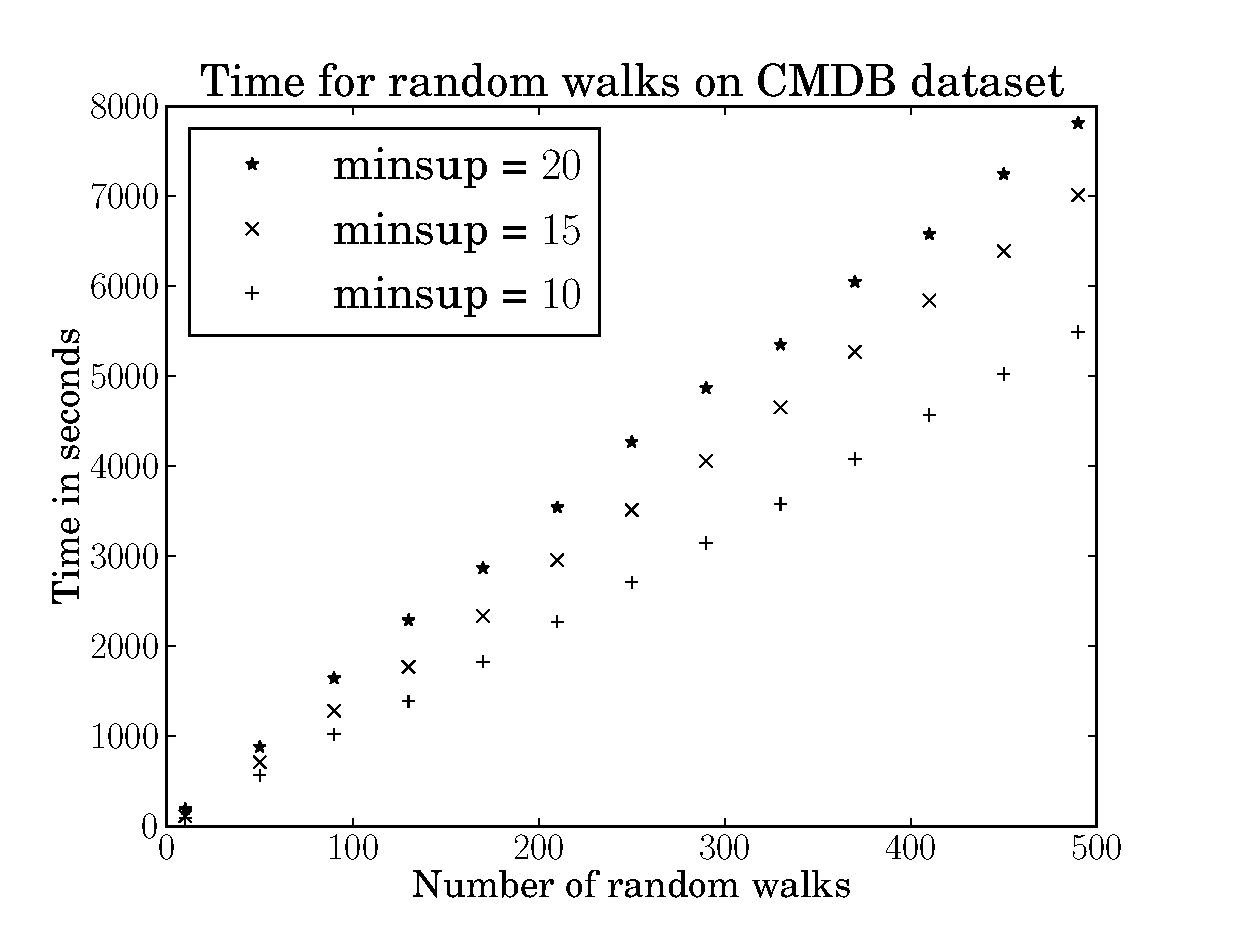
\includegraphics[width=2.5in]{cmdbtiming.eps}
	}
    \caption{CMDB: Time for different values of
	$minsup$}
    \label{fig:ge}
\end{figure}


\smallskip\noindent{\textit{Results}:} Figure \ref{fig:ge} shows the
time for random walks for different values of $minsup$ and $\alpha =
0.5$. Interesting, and somewhat counter-intuitively, the time increases
for higher minimum support values.  The reason is that with higher
minimum support, the random walk in the search space goes through the
nodes that have a large number of embeddings and it takes more time to
enumerate a single pattern.

The running time results above include a particular optimization that we
applied for CMDB graphs, given the large multiplicities of the different
labels. For such graphs, the 
support computation procedure can be improved by computing the sets of
equivalent vertices, i.e., vertices that have the same neighborhood and
are indistinguishable. The representative set $R(u)$ of all equivalent
vertices are equal, and thus it has to be computed only once.  In
abstract algebra terms, such vertices belong to an orbit of the
automorphism group of the graph \cite{orbits}.  So, we can prune the
candidate representative sets of all the vertices in an orbit by
matching the labels of any vertex in the orbit with the labels of
vertices in the candidate set. Computing the orbits of an arbitrary
graph is a hard problem. Several heuristics have been proposed to
compute the orbits of a graph \cite{Everett}.  We use a simple heuristic
to find subsets of vertices, common ancestor leaves (CAL) that are
guaranteed to be in the same orbit. These are the subset of leaves that
have the same label and are connected to a common ancestor.  CAL is a
subset $S \subseteq \vg$, such that $\forall u \in S$ and the following
three properties hold true: i) $|N(u)|=1$, ii) $\exists v \in \vg$,
$(v,u) \in \eg$, and  iii) $L(u) = l$  for some $l \in \Sigma$.
An example of CAL is set of all vertices labeled ``9 $\times$ process'' in
figure \ref{fig:gepatsB}; here 9 is the multiplicity of that label. 
CAL sets have to be computed once for every
candidate and this step had negligible impact on the overall run time. 


\begin{figure}[!h]
    \centerline{
    \subfloat[Pattern $A$] {
	\label{fig:gepatsA}
      \scalebox{0.6}{
        \begin{pspicture}(-2,-0.5)(3,5)	
          \begin{psmatrix}[rowsep=1,colsep=1]
          \Toval[name=n4]{running\_software} & & \\
             \Toval[name=n1]{windows\_service} & \Tcircle[name=n2]{iis} &
            \Toval[name=n3]{iisftpservice}\\
            \Tcircle[name=n5]{nt} & & \\
            \Toval[name=n6]{ip\_address} & \Toval[name=n7]{webvirtualhost} &
            \Toval[name=n8]{iiswebsite}
            %\Toval[name=n1]{business\_application} & \Toval[name=n2]{windows\_service}\\
            %\Tcircle[name=n3]{nt} & \\
            %\Toval[name=n5]{sqlserver} & \Toval[name=n4]{process}\\
            %& \Toval[name=n6]{windows\_service $\times$ 8}
          \end{psmatrix}
          \ncline{n1}{n4}
          \ncline{n1}{n2}
          \ncline{n2}{n3}
          \ncline{n2}{n5}
          \ncline{n2}{n7}
          \ncline{n1}{n5}
          \ncline{n1}{n4}
          \ncline{n6}{n5}
          \ncline{n7}{n6}
          \ncline{n7}{n8}
          \ncline{n3}{n8}
        \end{pspicture}
      }
	  }}
	\centerline{
    \subfloat[Pattern $B$] {
	\label{fig:gepatsB}
      \scalebox{0.5}{
        \begin{pspicture}(-2,-1)(4,7)	
          \begin{psmatrix}[rowsep=1,colsep=1]
            & \Toval[name=n1]{9 $\times$ process} & & \Toval[name=n2]{ip\_address} \\
            & \Toval[name=n3]{windows\_service} & \Tcircle[name=n4]{nt} &
            \Toval[name=n5]{ip\_address} \\
            \Toval[name=n6]{iisftpservice} & \Tcircle[name=n7]{iis} & &
            \Toval[name=n8]{webvirtualhost} \\
            & & \Toval[name=n9]{iisappool} & \\
            & \Toval[name=n10]{iisftpservice} & & \Toval[name=n11]{iiswebsite} \\
          \end{psmatrix}
        \ncline{n1}{n4}
        \ncline{n2}{n4}
        \ncline{n3}{n4}
        \ncline{n5}{n4}
        \ncline{n6}{n7}
        \ncline{n3}{n7}
        \ncline{n8}{n7}
        \ncline{n7}{n9}
        \ncline{n11}{n9}
        \ncline{n11}{n8}
        \ncline{n7}{n10}
        \ncline{n10}{n11}
        \ncline{n5}{n8}
        \end{pspicture}
      }
	  }}
    \caption{CMDB: Approximate Patterns}
    \label{fig:gepats}
  \end{figure}

\smallskip\noindent{\textit{Example Patterns}:}
Figure \ref{fig:gepats} shows maximal approximate
patterns from the real world CMDB graph. Both these patterns show
typical ``default'' 
configurations of the IT infrastructure in this company. They show the
connection between some services running on an NT server, and also the
web/ftp services.


\begin{figure}
    \centering
    \scalebox{0.6}{
    \begin{pspicture}(0,0)(3,5)
          \begin{psmatrix}[rowsep=1,colsep=1]
          & \Toval[name=n1]{running\_software} & \\
          \Toval[name=n2]{EnrichActImpl} & & \Toval[name=n3]{process}\\
          \Toval[name=n4]{process} & \Toval[name=n5]{nt} &
          \Toval[name=n6]{ip\_address}\\
          & \Toval[name=n7]{$8 \times process$} & \\
          \end{psmatrix}
          \ncline{n1}{n2}
          \ncline{n2}{n3}
          \ncline{n2}{n4}
          \ncline{n2}{n5}
          \ncline{n4}{n5}
          \ncline{n5}{n6}
          \ncline{n5}{n3}
          \ncline{n5}{n1}
          \ncline{n5}{n7}
    \end{pspicture}
    }
    \caption{Complete Enumeration Expensive}
    \label{fig:geex}
\end{figure}

To show the effectiveness of the pruning based on labels, we compared
the time taken to enumerate a single maximal pattern in $CMDB$ database.
We compared the time with and without label-based pruning.
Both the methods terminated the random walk with the maximal pattern
shown in Figure~\ref{fig:geex}.  
However, the total time taken to enumerate the pattern
without using any derived label is $18306$ secs whereas by using the
\combined label the total time reduced to only $15.5776$ secs. The huge
difference between the times arises due to the multiplicity effect in
$CMDB$ graphs.  



\subsection{Protein Structure Dataset (SCOP)}
SCOP (\url{scop.mrc-lmb.cam.ac.uk/scop/}) 
is a hierarchical classification of proteins based on structure
and sequence similarity. The four levels of hierarchy in this
classification are: class, fold, superfamily and family.  The $3D$
structure of a protein can be represented as an undirected graph with
the vertex labels being the amino acids, with an edge connecting two
nodes if the distance between the 
3D coordinates of the two amino acids (their
$\alpha$-Carbon atoms) is within a threshold (we use 7 Angstroms).
We constructed a database of
$100$ protein structures belonging to $5$ different families with $20$
proteins from each family. 
We chose the proteins from different levels in the SCOP hierarchy, and
we also focused on large proteins (those with more than 200 amino
acids). 
The 3D protein structures were downloaded from the
protein data bank (\url{http://www.rcsb.org/pdb}).  The database
can be considered as a single large graph with $100$ connected
components. 
For the SCOP dataset, the support is redefined as 
the number of proteins containing the pattern, i.e., 
even if a protein contains multiple embeddings we count them only once for the support.

\smallskip\noindent{\textit{Cost Matrix}:}
Since there are 20 different amino acids, we need a $20 \times 20$ cost
matrix. BLOSUM62~\cite{HH92} is a commonly used substitution matrix for aligning protein
sequences.  The $i,j$ entry in BLOSUM denotes the log-odd score
of substituting the amino acids $a_i$ and $a_j$, defined as
\begin{equation*}
    \label{eq:blosum}
    \matij{B}{i}{j} = \frac{1}{\lambda} 
	\log\frac{p_{ij}}{f_i \cdot f_j}
\end{equation*}
where $p_{ij}$ denotes the probability that  $a_i$ can be
substituted by $a_j$; 
$f_i$, $f_j$ denote the prior probabilities for observing the 
amino acids; and $\lambda$ is a constant. We compute $f_i$ and $f_j$
from the database, and then reconstruct $p_{ij}=f_if_j e^{\lambda
B_{i}}$. Next, we define the pair-wise amino acid cost matrix as
$\matij{C}{i}{j} = 1-\frac{p_{ij}}{p_{ii}}$, which ensures that
the diagonal entries are $\matij{C}{i}{i} =0$.

\begin{figure}[!ht]
	\centerline{
    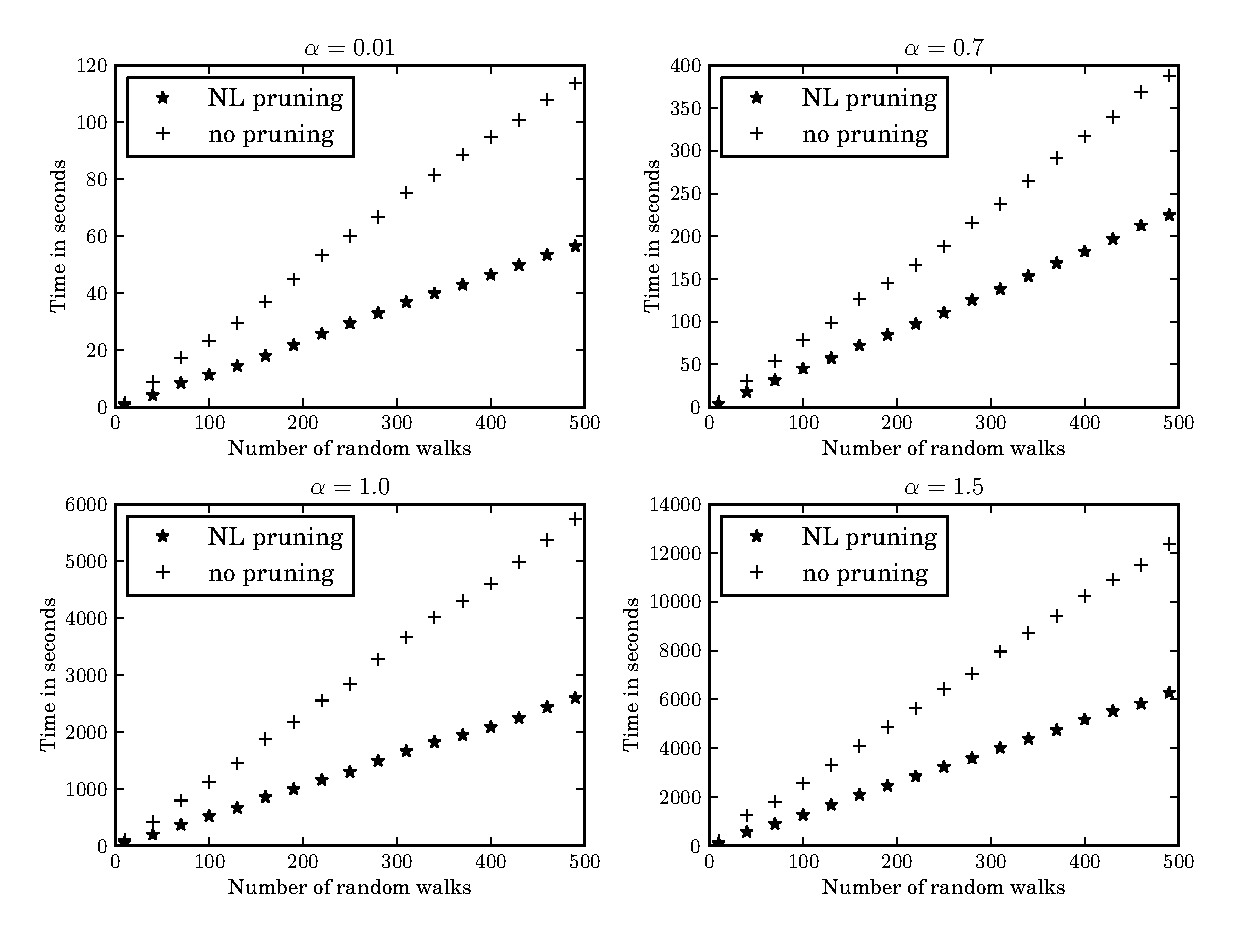
\includegraphics[width=3in]{5F20P.eps}
	}
	\caption{SCOP: Effect of $\alpha$ (increasing in 
	clockwise order from top right)}
    \label{fig:5F20P}
\end{figure}

\begin{figure}[!ht]
  \centerline{
    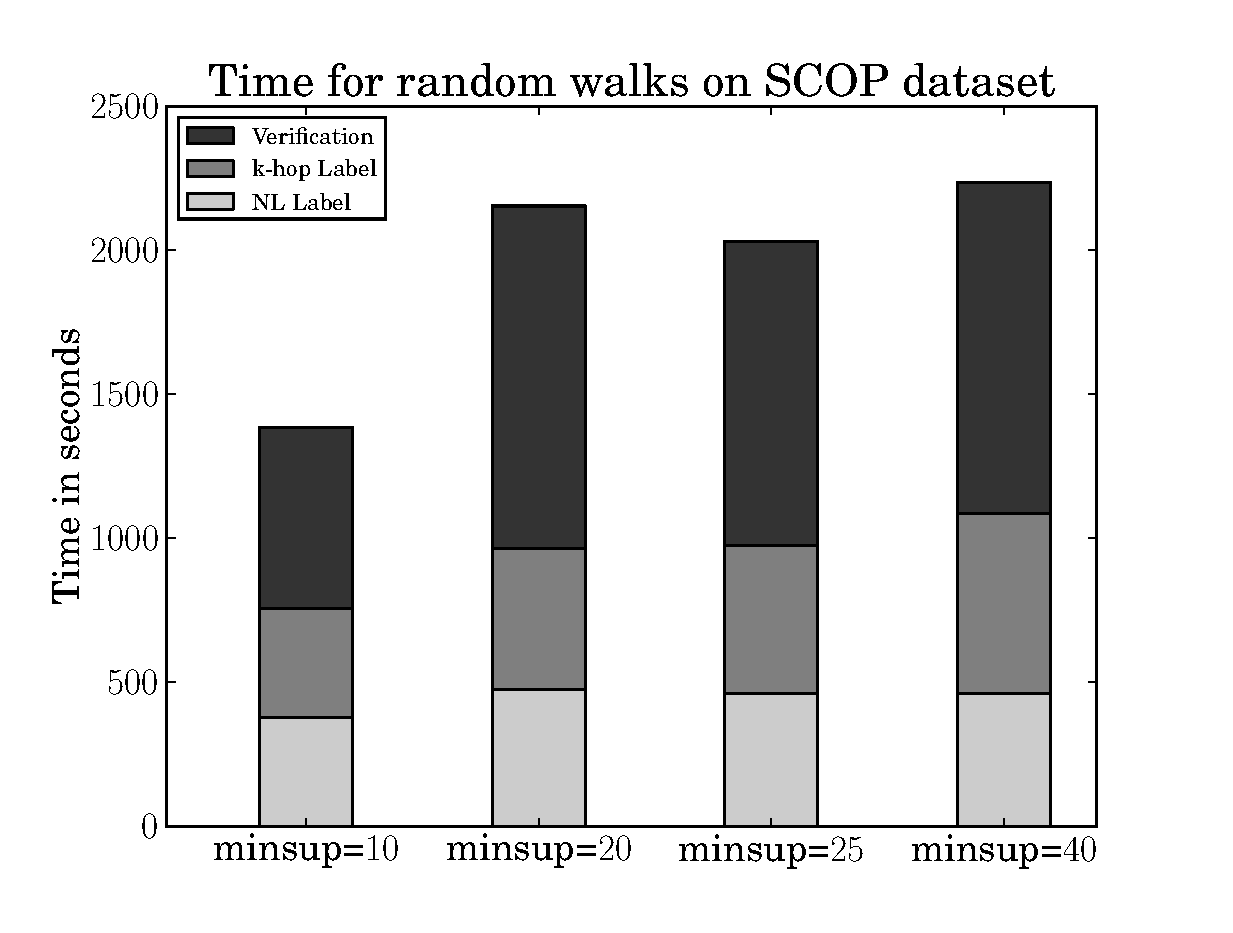
\includegraphics[width=2.5in]{scop_minsup.eps}
	}
	\caption{SCOP: Effect of $minsup$}
    \label{fig:5F20P_ft}
\end{figure}


\smallskip\noindent{\textit{Results}:}
Figure \ref{fig:5F20P} shows the time taken for enumerating approximate
maximal patterns for different values of $\alpha$ (with fixed $minsup =
20$). The plots show the time for random walks with and without the
label pruning. It can be seen that by using the label-based pruning the
time for random walks reduces significantly (by over 100\%).  As
expected, the time increases as the values of $\alpha$ increases, since
the number of isomorphisms clearly increases for a more relaxed (larger)
cost threshold.  When $\alpha = 0.01$, the patterns are exact as
$\matij{C}{i}{j} > \alpha$ $,\forall i \neq j$.

Figure \ref{fig:5F20P_ft} shows the time taken for $K=500$ random walks
for various values of $minsup$, but with a fixed $\alpha = 0.7$. The bar
plot shows time spent in \khop matching (Hops), \ncl matching
(Neighbors) and pattern verification (Enumeration). In general, the time
increases as the $minsup$ increases because the representative sets
$R(u)$ become larger. However, there is no fixed trend as the total time
depends on the regions of pattern space that the random walk explores.

\begin{figure}[!ht]
  \centerline{
    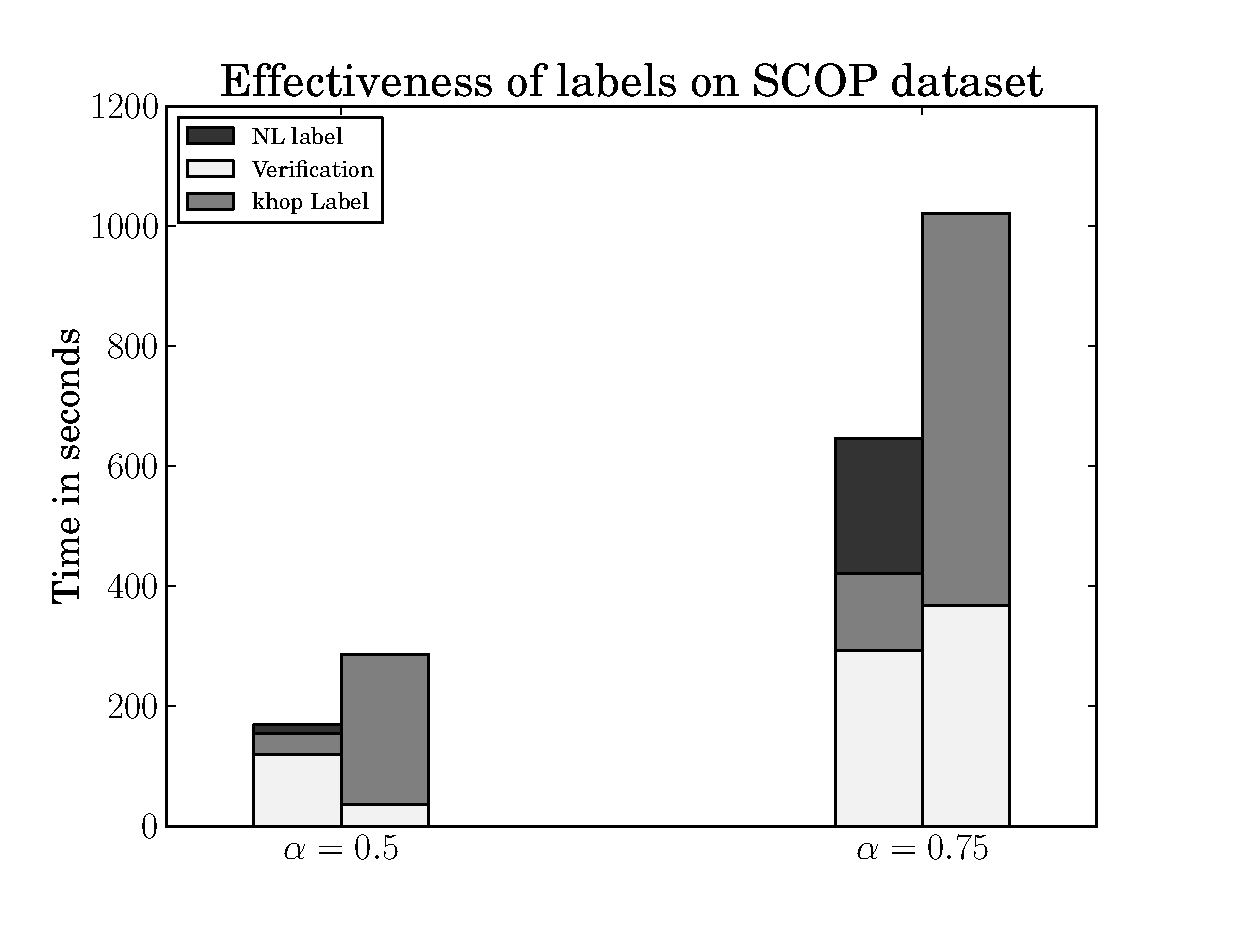
\includegraphics[width=2.5in]{scop_effectiveness.eps}
	}
	\caption{SCOP: Effectiveness of labels}
    \label{fig:D5F20P_eff}
\end{figure}

Figure~\ref{fig:D5F20P_eff} compares the effectiveness of the \combined
label (Neighbors) and \khop label (Hops) for different values of the
threshold $\alpha$ on the SCOP dataset.  For each value of $\alpha$, the
left bar shows the time with \combined label, whereas the right bar
shows the time using only the \khop label.  The \combined label clearly
reduces the time taken. In fact, it reduces the time for both the \khop
matching and the pattern verification steps, since \combined is very
effective in pruning the representative set.  This effect is best seen
for $\alpha = 0.75$, where the total time for the enumeration reduces
even though matching the neighbors takes more time compared to \khop
matching.  This shows the effectiveness of the \combined label versus
\khop label in isolation.

\begin{figure}[!ht]
  \centerline{
  \subfloat[Pattern $A$]{
    \label{fig:scopA}
    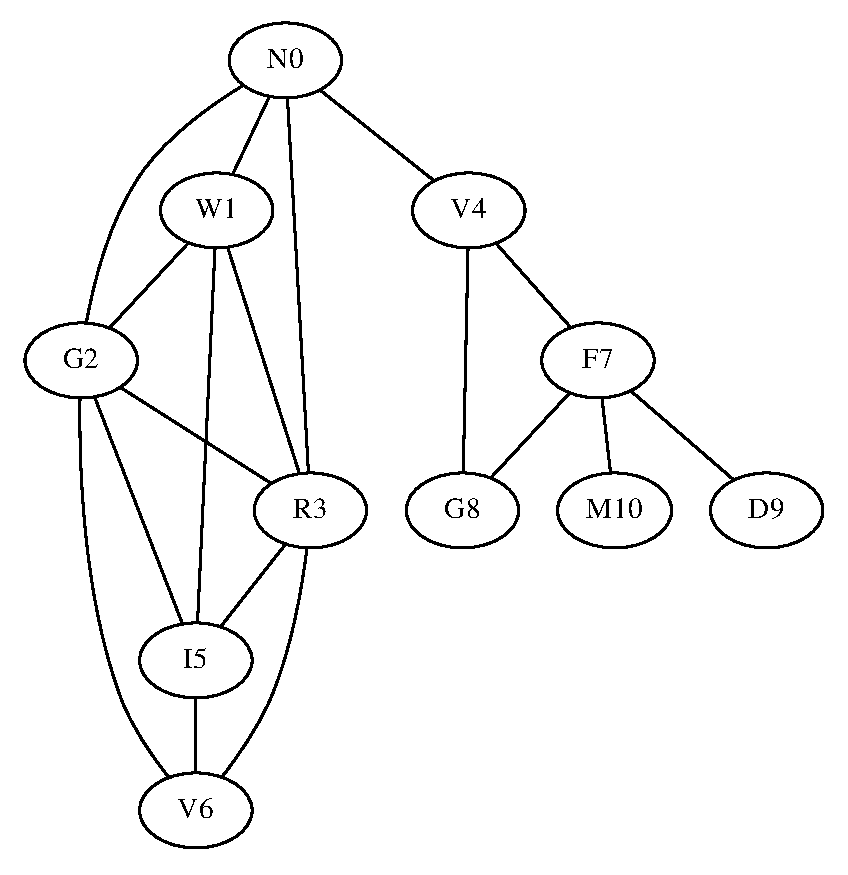
\includegraphics[width=1.5in,height=1.25in]{1ysw.pat.eps}
	}
  \subfloat[Pattern $B$]{
    \label{fig:scopB}
    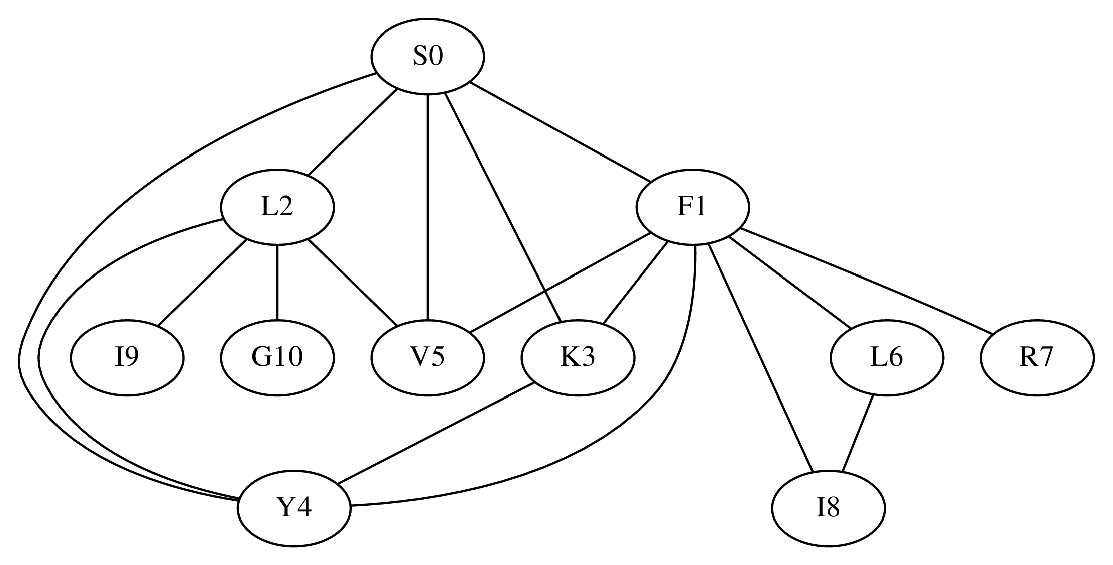
\includegraphics[width=1.5in,height=1.0in]{1r2e.pat.eps}
	}	
	}
	\centerline{
	\subfloat[Structural Motif $A$]{
    \label{fig:scopAS}
    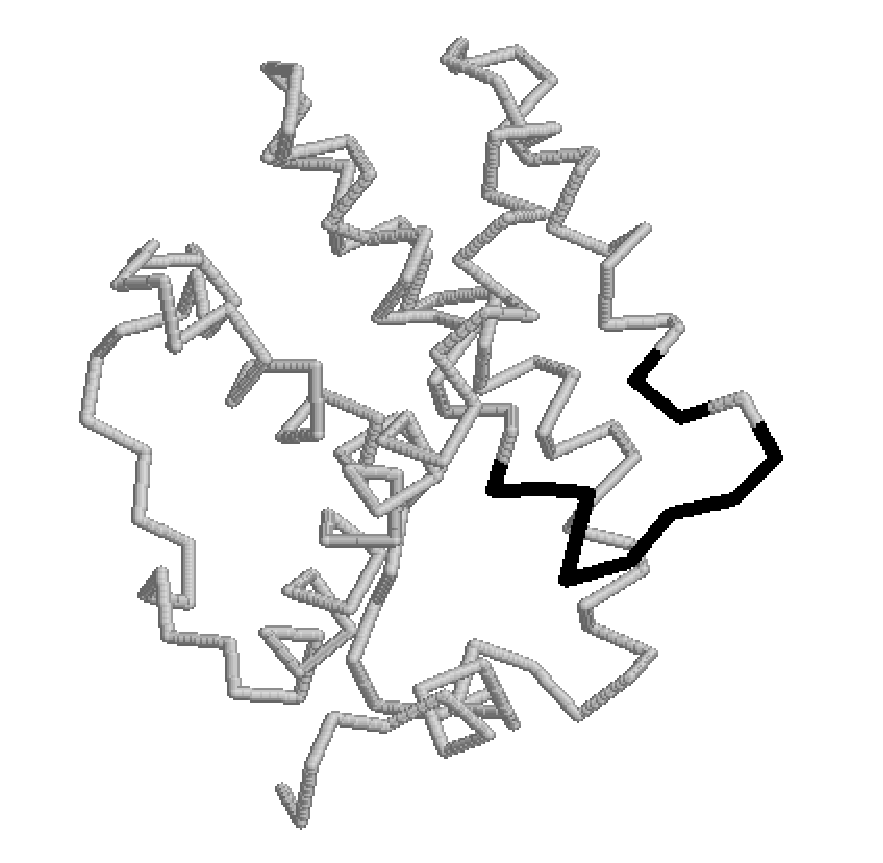
\includegraphics[width=1.5in,height=1.5in]{1ysw.eps}
	}
	\subfloat[Structural Motif $B$]{
    \label{fig:scopBS}
    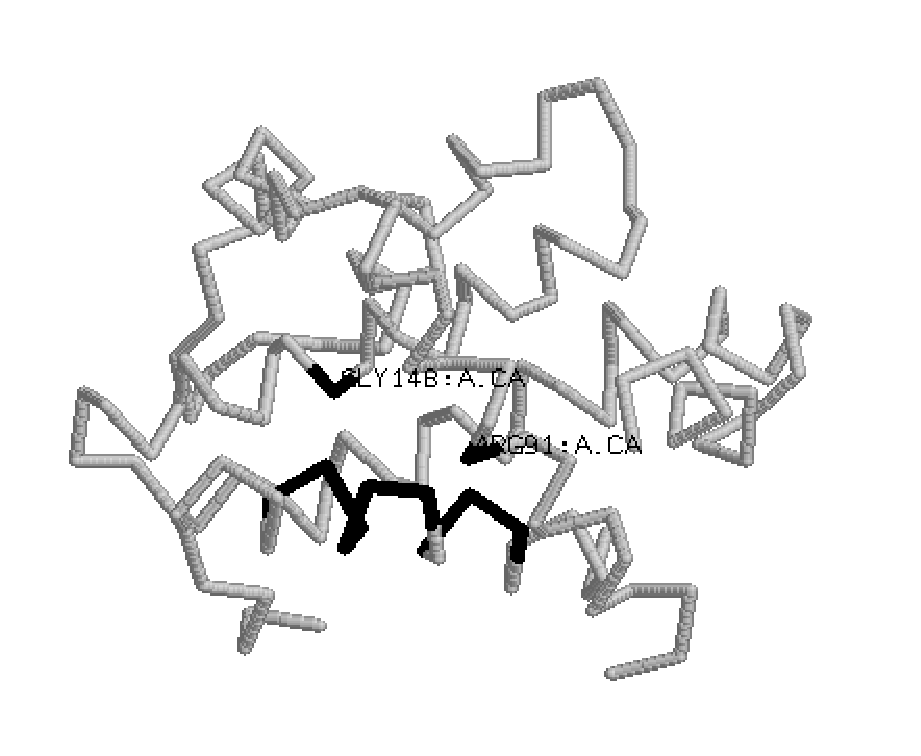
\includegraphics[width=1.5in,height=1.5in]{1r2e.eps}
	}
	}
	\caption{SCOP: Approximate Graph Patterns and their Structures}
	\label{fig:scoppats}
\end{figure}


\smallskip\noindent{\textit{Example Patterns}:}
Figure~\ref{fig:scoppats} shows examples of approximate protein graph
patterns and their corresponding 3D structure extracted from the SCOP
dataset.  For example, the graph in \ref{fig:scopA} appears in only one of
the families. This pattern occurs in 18 of the 20 members, and the
structure of one its occurrences, in protein PDB:1YSW, is shown in
\ref{fig:scopAS}. The common motif corresponds to the black colored
amino acids.  Another approximate pattern is shown in \ref{fig:scopB},
and its structure in PDB:1R2E is shown in \ref{fig:scopBS}; it has
support 19.  It is important to note that the cost of this isomorphism
is $C(\phi) = 0.4541$, indicating that exact isomorphism cannot find the
motif.

\subsection{Protein-Protein Interaction Network (PPI)} We ran
experiments on a yeast (Saccharomyces cerevisiae) PPI network. The list of
interacting proteins for yeast was downloaded from the DIP database
(\url{http://dip.doe-mbi.ucla.edu}). As seen in Table~\ref{tab:db}, the
PPI network has 4950 proteins and 16,515 interactions.  Unlike the other
datasets, each node in the PPI network essentially has a unique label,
which is the protein name.  

\smallskip\noindent{\textit{Cost Matrix}:} 
To construct the cost matrix for the protein network we consider the
similarity between the protein sequences for any two adjacent nodes.
Sequence similarity is obtained via the BLAST alignment
score~\cite{altschul90}, that returns the expected value (E-value) of
the match. A low E-value implies high similarity, thus we create a
binary cost matrix between the proteins by setting
$\matij{C}{p_i}{p_j} =0$ iff the proteins $p_i$ and $p_j$ have high
similarity, i.e., iff $E-value(p_i, p_j) \le \epsilon$. We empirically 
set $\epsilon = 0.003$.


\begin{figure}[!h]
	\centerline{
	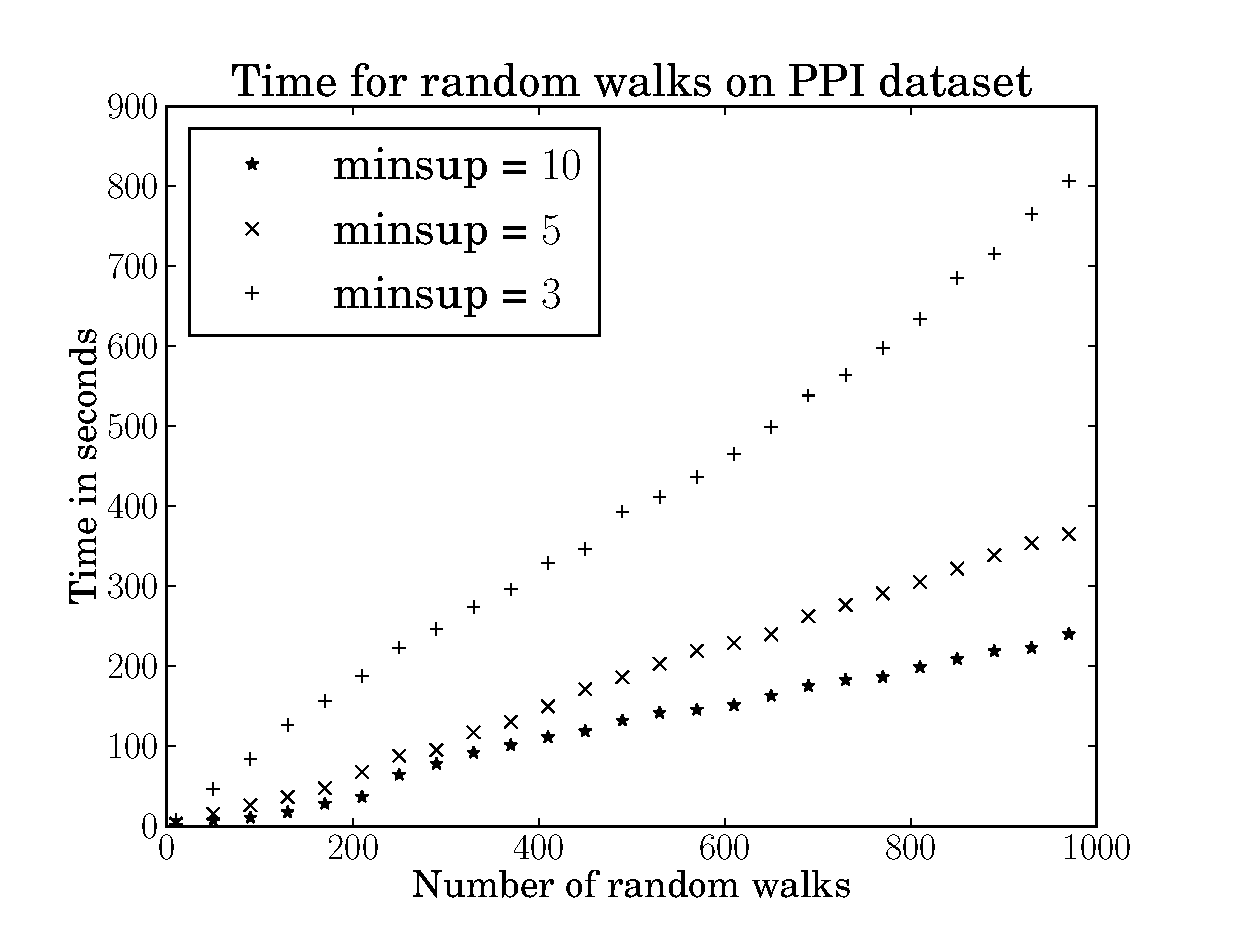
\includegraphics[width=2.5in]{ppi.eps}
	}
    \caption{PPI: Time for different values of $minsup$}
    \label{fig:ppiwalks}
\end{figure}

\smallskip\noindent{\textit{Results}:} Figure \ref{fig:ppiwalks} shows
the time for random walks in the yeast $PPI$ network for different values of
$minsup$.  It can be seen that the time for random walks decreases as
the support value increases.  One of the differences for the PPI graph
is that we do not utilize the \khop labels.  The complexity of matching
the \khop labels depends on the number of literals in the \khop label.
As each label(protein) is unique in the PPI graph, the number of
literals in the \khop label of a vertex $v$ in a PPI network is equal to
the number of vertices reachable in \khops. This increases the run time
for the \khop label matching.  Therefore, for mining PPI networks we use
only the \ncl labels.


\begin{figure}[!ht]
  \subfloat[Pattern $A$]{
    \label{fig:ppipatsA}
    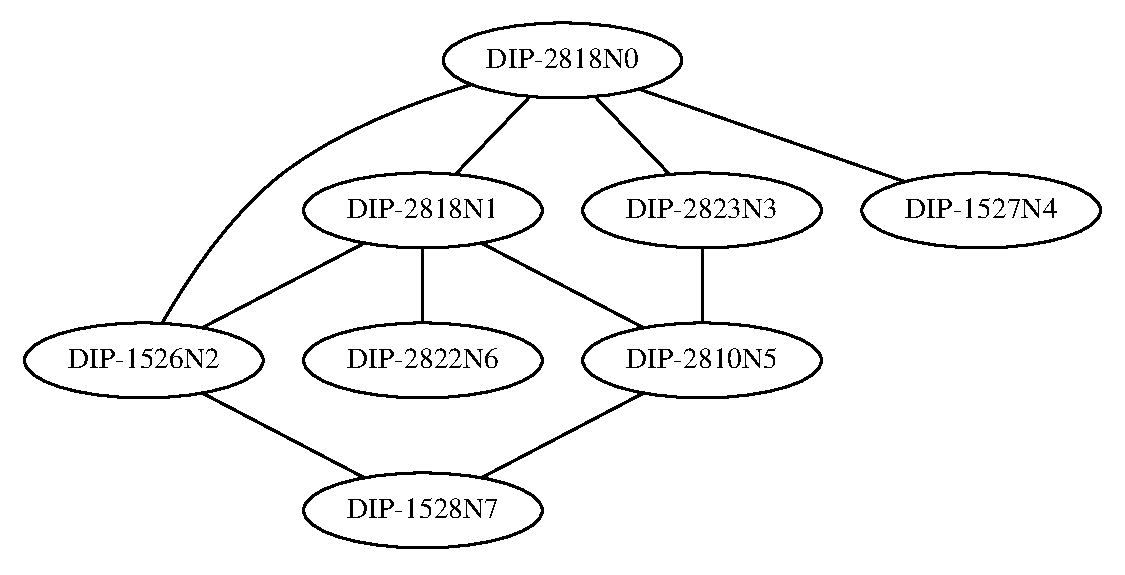
\includegraphics[width=2in]{ppipat2.eps}
	}\\
\subfloat[GO Terms for $A$]{
  % Table for the search space pruning
    \label{fig:ppipatsAT}
  \begin{tabular}{c|p{2in}}
GO Terms & Description\\
\hline
BP:0051603&      proteolysis involved in cellular protein catabolic
process\\
\hline
MF:0004298&      threonine-type endopeptidase activity\\
\hline
CC:0034515&      proteasome storage granule\\
  \end{tabular}
  %\label{subfig:match}
  } \\ 
  \subfloat[Pattern $B$]{
    \label{fig:ppipatsB}
    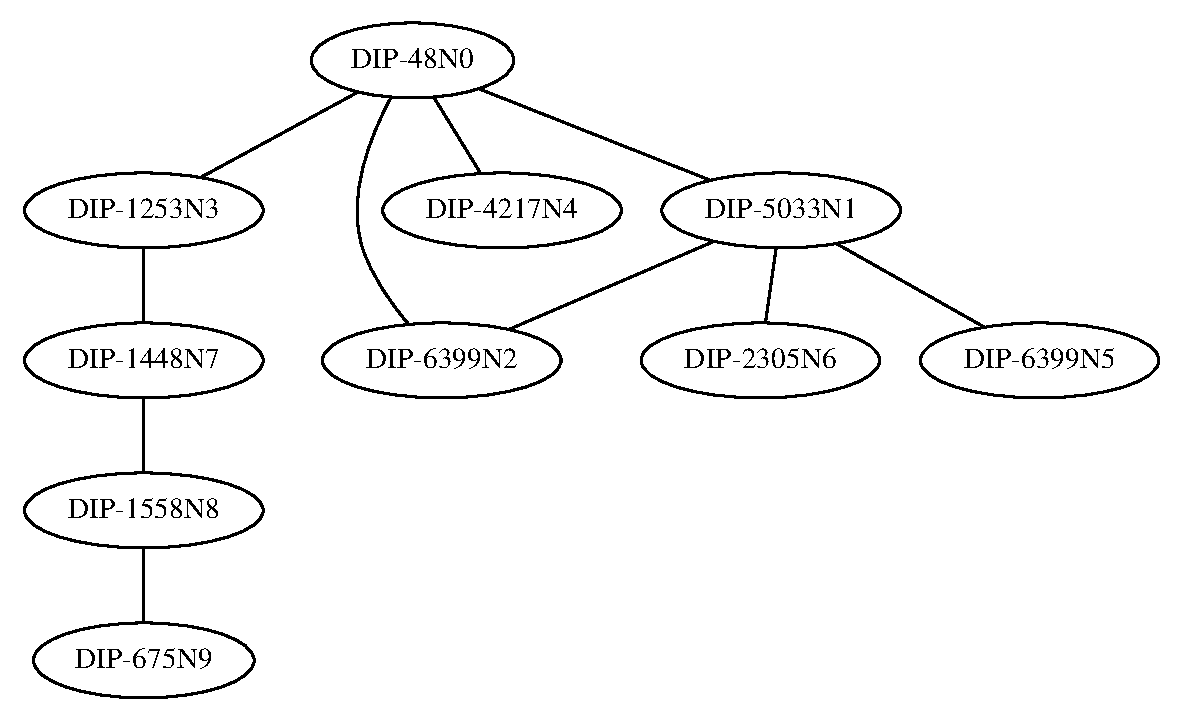
\includegraphics[width=2in]{ppipat1.eps}
	}\\
  \subfloat[GO Terms for $B$]{
    \label{fig:ppipatsBT}
  \begin{tabular}{c|p{2in}}
GO Terms & Description\\
\hline
BP:0004674  & protein serine/threonine kinase activity\\
\hline
MF:0016301   &   kinase activity\\
MF:0005524   &   ATP binding\\
  \end{tabular}
  }
    \caption{Approximate PPI Patterns and GO Enrichment}
    \label{fig:ppipats}
\end{figure}

\begin{comment}
\begin{figure}[!ht]
  \centerline{
  \subfloat[Pattern $A$]{
    \label{fig:ppipatsA}
    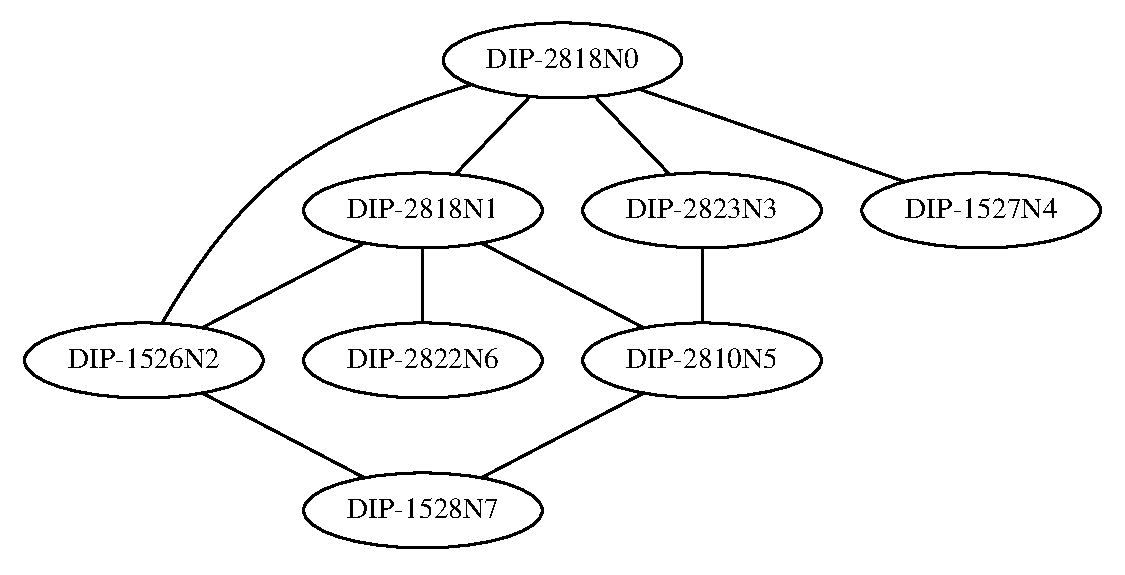
\includegraphics[width=2in]{ppipat2.eps}
	}}
	\centerline{
  \subfloat[GO Terms for $A$]{
    \label{fig:ppipatsAT}
  \small
  \begin{tabular}{c|p{2in}}
GO Terms & Description\\
\hline
BP:0051603&      proteolysis involved in cellular protein catabolic
process\\
\hline
MF:0004298&      threonine-type endopeptidase activity\\
\hline
CC:0034515&      proteasome storage granule\\
  \end{tabular}
  }}
  \centerline{
  \subfloat[Pattern $B$]{
    \label{fig:ppipatsB}
    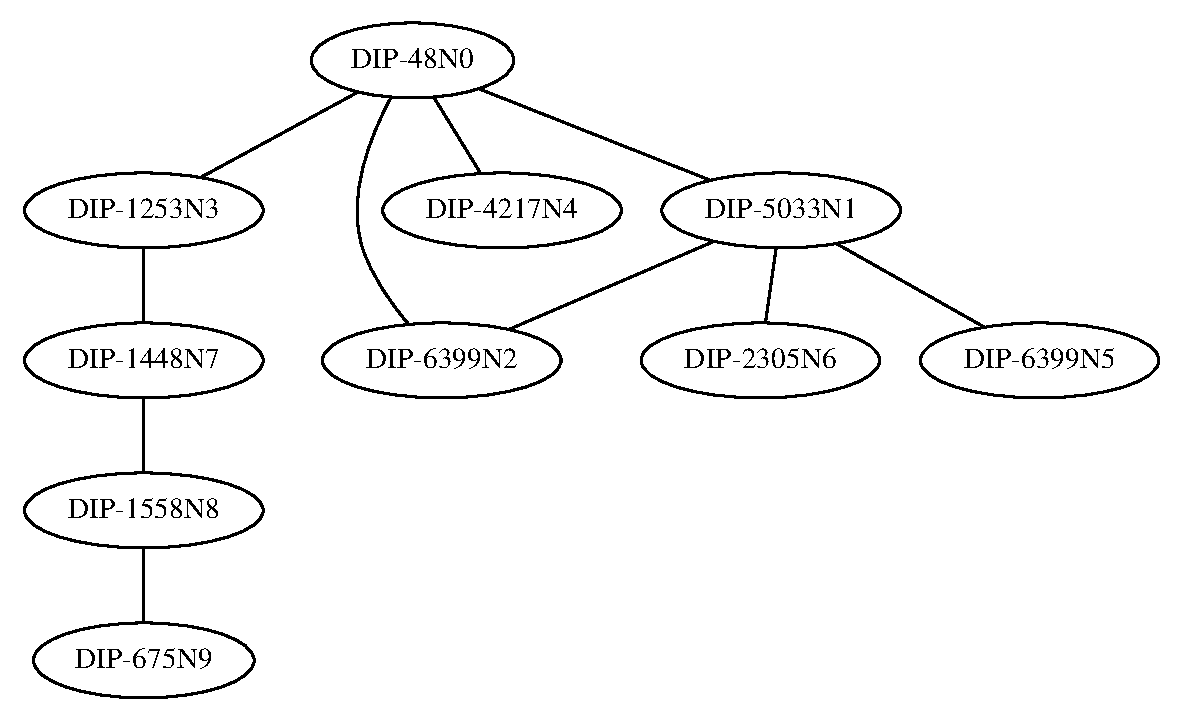
\includegraphics[width=2in]{ppipat1.eps}
	}}
	\centerline{
  \subfloat[GO Terms for $B$]{
    \label{fig:ppipatsBT}
  \small
  \begin{tabular}{c|p{2in}}
GO Terms & Description\\
\hline
BP:0004674  & protein serine/threonine kinase activity\\
\hline
MF:0016301   &   kinase activity\\
MF:0005524   &   ATP binding\\
  \end{tabular}
  }}
    \caption{Approximate PPI Patterns and GO Enrichment}
    \label{fig:ppipats}
\end{figure}
\end{comment}

\smallskip\noindent{\textit{Example Patterns}:}
Figures~\ref{fig:ppipatsA} and \ref{fig:ppipatsB} show two of the mined
maximal frequent approximate patterns (using $minsup=5$). The proteins
are labeled with their DIP identifiers (e.g., DIP-2818N); the last
number in the label is just a sequential node id.  It is worth
emphasizing that exact subgraph isomorphism would not yield any patterns
in this dataset, since each label is unique. However, since we allow a
protein to be replaced by a similar protein via the cost matrix \Cs,
we obtain interesting approximate patterns. To judge the quality of the
mined patterns we use the gene ontology (GO;
\url{www.geneontology.org}), which comprises three structured,
controlled vocabularies (ontologies) that describe gene products in
terms of their associated biological processes (BP), molecular functions
(MF), and cellular components (CC).  For each of the mined approximate
patterns we obtain the set of all the GO terms common to all proteins in
the pattern. This serves as an external validation of the mined results,
since common terms imply meaningful biological relationships among the
proteins.  Figure~\ref{fig:ppipatsAT} shows the common GO terms for
pattern $A$.  This subgraph comprises proteins involved in proteolysis
as the biological process, i.e., they act as enzymes that lead to the
breakdown of other proteins into amino acids. Their molecular function
is endopeptidase activity, i.e., breakdown of peptide bonds of
non-terminal amino acids, in particular the amino acid Threonine.  These
proteins are located in the proteasome storage granule, and most likely
comprise a protein complex (proteasome) -- a molecular machine --
that digests proteins into amino acids.  The common GO terms for pattern
$B$ in Figure~\ref{fig:ppipatsBT} indicate that the proteins function as
Kinases, proteins that are responsible for adding a phosphate to an
amino acid. The biological process is Phosphorylation, the
post-translational modification of proteins corresponding to adding a
phosphate, in particular modifying amino acids Serine and Threonine. 

\section{Related Work} 
\label{sec:relatedwork}

In the past, many algorithms have been proposed to mine subgraphs from a
given database of graphs. These algorithms can be mainly divided in to
two classes depending on how the candidate patterns are generated.
Algorithms like those in \cite{IWM03,FSG01,HWP03} are Apriori
based methods, i.e., a candidate pattern of size $k+1$ is generated by
combining two frequent graphs of size $k$ that have a common $k-1$ sized
subgraph.  Algorithms like those in \cite{gSpan},
on the other hand, belong to the class of pattern growth algorithms in
which a candidate pattern is generated by extending a frequent pattern
with another edge.
Sampling approaches like those proposed in
\cite{2009-graphsampling,2012-kais,RAM2008} mine a representative set of
maximal patterns from a database of graphs or a single graph; they are
especially effective in large real-world graphs where complete graph
mining is practically infeasible.

Mining subgraphs from a single graph is a related problem which is
surprisingly difficult compared to mining from a database of graphs.  In
\cite{kuramochi2005ffp}, they defined the support of a pattern
in a single graph as the maximum number of edge disjoint isomorphisms,
which is itself an $NP$-Hard problem.  In \cite{fiedler2007support}, they
proposed a definition of support based on overlapping ancestor
isomorphisms.  In \cite{2012-kais}, we proposed
CMDB-Miner\xspace to mine frequent patterns from a single large graph.
Support of a pattern is defined as the maximum flow in an appropriately
constructed flow network with capacities. This method estimates the
support of a pattern without enumerating its isomorphisms. 
%The authors
%also proposed methods to summarize the maximal frequent patterns
%extracted from the graph. In \cite{li2010dessin}, they proposed an
%algorithm to extract frequent patterns from dense graphs. It uses
%$GADDI$ index proposed in \cite{Gaddi2009} to efficiently extract the
%isomorphisms of a subgraph. 

There has been little work in approximate subgraph mining.  In
\cite{gapprox}, they proposed $gApprox$ to mine approximate frequent
subgraphs.  The degree of approximation between a pattern and its
isomorphism includes label mismatches and missing edges. The search
space is explored in a depth first order and the support of a pattern is
computed by enumerating all its isomorphisms. This approach is not
feasible for large graphs with label multiplicities as there are
potentially an exponential number of isomorphisms \cite{2012-kais}.  In
\cite{JiaZH11}, they proposed APGM to approximate frequent subgraphs
from a database of graphs. The method is similar to the $gApprox$
method, with the main difference being that 
 the entire $1$-hop neighborhood of the current embeddings
is explored to enumerate all extensions of the frequent pattern and
their corresponding embeddings, whereas $gApprox$ enumerates the
embeddings for a single extension in each step.  
However, they store the complete set of approximate embeddings of the
current frequent pattern, which can be a problem. 
In \cite{SpeedUpFAS},
the authors proposed strategies to speed up the existing approximate
mining algorithms, by limiting the number of candidates and also the
number of duplicate checks performed. They assume that the underlying
algorithm takes care of the label and/or edge mismatches.  In
\cite{RAM2008}, they proposed a randomized algorithm to mine approximate
patterns from a database graphs. This method only handles edge
mismatches and not label costs.
%an edge in the approximate pattern is required to have at least a given
%number of occurrences. 

Graph querying is another problem that is related to
subgraph mining. The goal is to find matches of a given query graph in a
single graph or database of graphs.  In \cite{TALE}, they proposed an
indexing method to extract the approximate occurrences of a given graph
query in large graph databases.  
%The algorithm proposed in
%\cite{yan.icde:2006} extracts selective fragments from the query graph
%and queries against an index constructed from the fragments of the
%database graphs. 
In \cite{RandomMatching}, they proposed a polynomial
time algorithm for detecting isomorphism between spectrally
distinguishable graphs. An isomorphism, if it exists, 
is obtained by matching
the steady state vectors of Markov chains in both the graphs.  
%In
%\cite{BerettiIndexing}, they proposed indexing and retrieval methods for
%graph models. 
The problem with the indexing approaches is that
they are efficient in retrieving a single match for the query graph but
fail at retrieving all matches, and thus are not suited to mine frequent
patterns. Furthermore, they assume that the query is given, and thus they
do not perform pattern enumeration as required in graph mining.

%Frequent pattern mining algorithms usually return a large number of
%patterns and interpreting them is a big challenge. This is especially
%true if the output is presented to a human user for further analysis.
%Sampling approaches like those proposed in
%\cite{2009-graphsampling,2012-kais,RAM2008} mine a representative set of
%maximal patterns from a database of graphs or a single graph. 
%In our work, we perform a random walk in the search space
%to enumerate a maximal pattern.

%The concept of using derived labels based on the
%structure and the attributes is frequently used in detecting graph
%isomorphism \cite{zampelli} and computing graph kernels
%\cite{shervashidzeJmlr,shervashidzeNips}. 
%Our methods to prune representative sets are somewhat similar to
%the wiesfieler lehman kernel to test isomorphism between two graphs
%$G_1$ and $G_2$ \cite{weisfeiler}, where after every iteration the labels are
%sorted and renamed with a different string in such a way that the pairwise
%relationship is maintained. $G_1$ is not isomorphic to $G_2$ 
%if the label set of the graphs differ. The specifics of how and what
%information we update is different, and also we use the information for
%subgraph isomorphism instead of graph isomorphism.


% conclusions and future work
\section{Discussions and Conclusions}

We presented an effective approach to mine approximate frequent subgraph
patterns from a single large graph database in the presence of
a label cost matrix.

There are two main parameters in our method: $K$, the number of random
walks, and $\alpha$ the cost threshold. The value of $K$ is directly
proportional to the number of maximal approximate patterns we desire,
and is relatively easy to set.
On the other hand, choosing an appropriate value of
$\alpha$ is very important as it affects the quality of
patterns mined. Depending on the application domain
and the purpose of the graph mining, let $t$ be the number of
vertices in the pattern for which we allow label mismatches
in the subgraph isomorphism. One reasonable value of
$\alpha$ is $t \times IMQ$ where $IMQ$ is the inter-quartile mean
i.e., the mean of the entries between the first quartile ( $25^{th}$
percentile) and the third quartile ( $75^{th}$ percentile)
of the entries in the cost matrix arranged in sorted order. 
$t$ can be chosen by first
enumerating maximal patterns with $\alpha = 0$ and computing the 
average size $m$ of the maximal patterns mined from the graph.
The value of $t$ then is a fraction of the average size $m$.
Care has to be taken not to choose a very large $\alpha$ as it leads to
patterns of poor quality and also increases the run time of the
algorithm significantly as can be seen in the Figure \ref{fig:5F20P}.

In terms of future work, we plan to increase the efficiency of our
method by exploiting parallelism. Obviously different walks can be
carried out in parallel. However, more interesting is the
parallelization of the approximate isomorphism generation and
label-based pruning steps, including verification. We also
want to explore the idea of label based pruning for more
general definitions of approximate isomorphism including 
edge mismatches.



\small
\bibliographystyle{abbrv}
\bibliography{./references/relevant}  % sigproc.bib is the name of the Bibliography in this case

\end{document}
